\documentclass{llncs}
%%%%%%%%%%%%%%%%%%%%%%
%%%%   PACKAGES   %%%%
%%%%%%%%%%%%%%%%%%%%%%
\usepackage{makeidx}
\usepackage{amsmath}
\usepackage{amssymb}
\usepackage{stmaryrd}
\usepackage{graphicx}
\usepackage{subfigure}
\usepackage{latexsym}
\usepackage{url}
\usepackage{color}
\usepackage{isabelle}
\usepackage{isabellesym}
\usepackage{theorem}
\usepackage[linesnumbered,ruled,vlined]{algorithm2e}
%%%%%%%%%%%%%%%%%%%%%%%%%%%%
%For Isabelle code
\newlength{\fminilength}
\newsavebox{\fminibox}
\newenvironment{fmini}[1][\linewidth]
  {\setlength{\fminilength}{#1\fboxsep-2\fboxrule}%
   \vspace{2ex}\noindent\begin{lrbox}{\fminibox}\begin{minipage}{\fminilength}%
   \mbox{ }\hfill\vspace{-2.5ex}}%
  {\end{minipage}\end{lrbox}\vspace{1ex}\hspace{0ex}%
   \framebox{\usebox{\fminibox}}}

\newenvironment{specification}
{\noindent\scriptsize
\tt\begin{fmini}\begin{tabbing}X\=X12345\=XXXX\=XXXX\=XXXX\=XXXX\=XXXX
\=\+\kill} {\end{tabbing}\normalfont\end{fmini}}
\def \twoSpaces {\ \ }
\def \oneSpace {\ }
\def \eqc {= }
\def \andc {\wedge }
\def \negc {\neg }
\def \orc {\vee }
\def \alt {$/\backslash$ }
\def \cat {\symbol{94}}

\def \dbRight {$\backslash\backslash$}
\def \iInv {iInv}
\def \iR {iR}
%%%%%%%%%%%%%%%%%%%%%%%%%%%%

%%%%%%%%%%%%%%%%%%%%%%%%%%%%
%for comments
\newcommand\JP[1]{\textcolor{magenta}{JP: #1}}
\newcommand\lyj[1]{\textcolor{green}{lyj: #1}}
%%%%%%%%%%%%%%%%%%%%%%%%%%%

%%%%%%%%%%%%%%%%%%%%%%%%%%%
% Additional math operators
%%%%%%%%%%%%%%%%%%%%%%%%%%%

\usepackage[colorlinks,
            linkcolor=black,
            anchorcolor=black,
            citecolor=blue,
            urlcolor=black,
            bookmarks=true
            ]{hyperref}

% Macros for Scientific Word 2.5 documents saved with the LaTeX filter.
%Copyright (C) 1994-95 TCI Software Research, Inc.
\typeout{TCILATEX Macros for Scientific Word 2.5 <22 Dec 95>.}
\typeout{NOTICE:  This macro file is NOT proprietary and may be 
freely copied and distributed.}
%
\makeatletter
%
%%%%%%%%%%%%%%%%%%%%%%
% macros for time
\newcount\@hour\newcount\@minute\chardef\@x10\chardef\@xv60
\def\tcitime{
\def\@time{%
  \@minute\time\@hour\@minute\divide\@hour\@xv
  \ifnum\@hour<\@x 0\fi\the\@hour:%
  \multiply\@hour\@xv\advance\@minute-\@hour
  \ifnum\@minute<\@x 0\fi\the\@minute
  }}%

%%%%%%%%%%%%%%%%%%%%%%
% macro for hyperref
\@ifundefined{hyperref}{\def\hyperref#1#2#3#4{#2\ref{#4}#3}}{}

% macro for external program call
\@ifundefined{qExtProgCall}{\def\qExtProgCall#1#2#3#4#5#6{\relax}}{}
%%%%%%%%%%%%%%%%%%%%%%
%
% macros for graphics
%
\def\FILENAME#1{#1}%
%
\def\QCTOpt[#1]#2{%
  \def\QCTOptB{#1}
  \def\QCTOptA{#2}
}
\def\QCTNOpt#1{%
  \def\QCTOptA{#1}
  \let\QCTOptB\empty
}
\def\Qct{%
  \@ifnextchar[{%
    \QCTOpt}{\QCTNOpt}
}
\def\QCBOpt[#1]#2{%
  \def\QCBOptB{#1}
  \def\QCBOptA{#2}
}
\def\QCBNOpt#1{%
  \def\QCBOptA{#1}
  \let\QCBOptB\empty
}
\def\Qcb{%
  \@ifnextchar[{%
    \QCBOpt}{\QCBNOpt}
}
\def\PrepCapArgs{%
  \ifx\QCBOptA\empty
    \ifx\QCTOptA\empty
      {}%
    \else
      \ifx\QCTOptB\empty
        {\QCTOptA}%
      \else
        [\QCTOptB]{\QCTOptA}%
      \fi
    \fi
  \else
    \ifx\QCBOptA\empty
      {}%
    \else
      \ifx\QCBOptB\empty
        {\QCBOptA}%
      \else
        [\QCBOptB]{\QCBOptA}%
      \fi
    \fi
  \fi
}
\newcount\GRAPHICSTYPE
%\GRAPHICSTYPE 0 is for TurboTeX
%\GRAPHICSTYPE 1 is for DVIWindo (PostScript)
%%%(removed)%\GRAPHICSTYPE 2 is for psfig (PostScript)
\GRAPHICSTYPE=\z@
\def\GRAPHICSPS#1{%
 \ifcase\GRAPHICSTYPE%\GRAPHICSTYPE=0
   \special{ps: #1}%
 \or%\GRAPHICSTYPE=1
   \special{language "PS", include "#1"}%
%%%\or%\GRAPHICSTYPE=2
%%%  #1%
 \fi
}%
%
\def\GRAPHICSHP#1{\special{include #1}}%
%
% \graffile{ body }                                  %#1
%          { contentswidth (scalar)  }               %#2
%          { contentsheight (scalar) }               %#3
%          { vertical shift when in-line (scalar) }  %#4
\def\graffile#1#2#3#4{%
%%% \ifnum\GRAPHICSTYPE=\tw@
%%%  %Following if using psfig
%%%  \@ifundefined{psfig}{\input psfig.tex}{}%
%%%  \psfig{file=#1, height=#3, width=#2}%
%%% \else
  %Following for all others
  % JCS - added BOXTHEFRAME, see below
    \leavevmode
    \raise -#4 \BOXTHEFRAME{%
        \hbox to #2{\raise #3\hbox to #2{\null #1\hfil}}}%
}%
%
% A box for drafts
\def\draftbox#1#2#3#4{%
 \leavevmode\raise -#4 \hbox{%
  \frame{\rlap{\protect\tiny #1}\hbox to #2%
   {\vrule height#3 width\z@ depth\z@\hfil}%
  }%
 }%
}%
%
\newcount\draft
\draft=\z@
\let\nographics=\draft
\newif\ifwasdraft
\wasdraftfalse

%  \GRAPHIC{ body }                                  %#1
%          { draft name }                            %#2
%          { contentswidth (scalar)  }               %#3
%          { contentsheight (scalar) }               %#4
%          { vertical shift when in-line (scalar) }  %#5
\def\GRAPHIC#1#2#3#4#5{%
 \ifnum\draft=\@ne\draftbox{#2}{#3}{#4}{#5}%
  \else\graffile{#1}{#3}{#4}{#5}%
  \fi
 }%
%
\def\addtoLaTeXparams#1{%
    \edef\LaTeXparams{\LaTeXparams #1}}%
%
% JCS -  added a switch BoxFrame that can 
% be set by including X in the frame params.
% If set a box is drawn around the frame.

\newif\ifBoxFrame \BoxFramefalse
\newif\ifOverFrame \OverFramefalse
\newif\ifUnderFrame \UnderFramefalse

\def\BOXTHEFRAME#1{%
   \hbox{%
      \ifBoxFrame
         \frame{#1}%
      \else
         {#1}%
      \fi
   }%
}


\def\doFRAMEparams#1{\BoxFramefalse\OverFramefalse\UnderFramefalse\readFRAMEparams#1\end}%
\def\readFRAMEparams#1{%
 \ifx#1\end%
  \let\next=\relax
  \else
  \ifx#1i\dispkind=\z@\fi
  \ifx#1d\dispkind=\@ne\fi
  \ifx#1f\dispkind=\tw@\fi
  \ifx#1t\addtoLaTeXparams{t}\fi
  \ifx#1b\addtoLaTeXparams{b}\fi
  \ifx#1p\addtoLaTeXparams{p}\fi
  \ifx#1h\addtoLaTeXparams{h}\fi
  \ifx#1X\BoxFrametrue\fi
  \ifx#1O\OverFrametrue\fi
  \ifx#1U\UnderFrametrue\fi
  \ifx#1w
    \ifnum\draft=1\wasdrafttrue\else\wasdraftfalse\fi
    \draft=\@ne
  \fi
  \let\next=\readFRAMEparams
  \fi
 \next
 }%
%
%Macro for In-line graphics object
%   \IFRAME{ contentswidth (scalar)  }               %#1
%          { contentsheight (scalar) }               %#2
%          { vertical shift when in-line (scalar) }  %#3
%          { draft name }                            %#4
%          { body }                                  %#5
%          { caption}                                %#6


\def\IFRAME#1#2#3#4#5#6{%
      \bgroup
      \let\QCTOptA\empty
      \let\QCTOptB\empty
      \let\QCBOptA\empty
      \let\QCBOptB\empty
      #6%
      \parindent=0pt%
      \leftskip=0pt
      \rightskip=0pt
      \setbox0 = \hbox{\QCBOptA}%
      \@tempdima = #1\relax
      \ifOverFrame
          % Do this later
          \typeout{This is not implemented yet}%
          \show\HELP
      \else
         \ifdim\wd0>\@tempdima
            \advance\@tempdima by \@tempdima
            \ifdim\wd0 >\@tempdima
               \textwidth=\@tempdima
               \setbox1 =\vbox{%
                  \noindent\hbox to \@tempdima{\hfill\GRAPHIC{#5}{#4}{#1}{#2}{#3}\hfill}\\%
                  \noindent\hbox to \@tempdima{\parbox[b]{\@tempdima}{\QCBOptA}}%
               }%
               \wd1=\@tempdima
            \else
               \textwidth=\wd0
               \setbox1 =\vbox{%
                 \noindent\hbox to \wd0{\hfill\GRAPHIC{#5}{#4}{#1}{#2}{#3}\hfill}\\%
                 \noindent\hbox{\QCBOptA}%
               }%
               \wd1=\wd0
            \fi
         \else
            %\show\BBB
            \ifdim\wd0>0pt
              \hsize=\@tempdima
              \setbox1 =\vbox{%
                \unskip\GRAPHIC{#5}{#4}{#1}{#2}{0pt}%
                \break
                \unskip\hbox to \@tempdima{\hfill \QCBOptA\hfill}%
              }%
              \wd1=\@tempdima
           \else
              \hsize=\@tempdima
              \setbox1 =\vbox{%
                \unskip\GRAPHIC{#5}{#4}{#1}{#2}{0pt}%
              }%
              \wd1=\@tempdima
           \fi
         \fi
         \@tempdimb=\ht1
         \advance\@tempdimb by \dp1
         \advance\@tempdimb by -#2%
         \advance\@tempdimb by #3%
         \leavevmode
         \raise -\@tempdimb \hbox{\box1}%
      \fi
      \egroup%
}%
%
%Macro for Display graphics object
%   \DFRAME{ contentswidth (scalar)  }               %#1
%          { contentsheight (scalar) }               %#2
%          { draft label }                           %#3
%          { name }                                  %#4
%          { caption}                                %#5
\def\DFRAME#1#2#3#4#5{%
 \begin{center}
     \let\QCTOptA\empty
     \let\QCTOptB\empty
     \let\QCBOptA\empty
     \let\QCBOptB\empty
     \ifOverFrame 
        #5\QCTOptA\par
     \fi
     \GRAPHIC{#4}{#3}{#1}{#2}{\z@}
     \ifUnderFrame 
        \nobreak\par #5\QCBOptA
     \fi
 \end{center}%
 }%
%
%Macro for Floating graphic object
%   \FFRAME{ framedata f|i tbph x F|T }              %#1
%          { contentswidth (scalar)  }               %#2
%          { contentsheight (scalar) }               %#3
%          { caption }                               %#4
%          { label }                                 %#5
%          { draft name }                            %#6
%          { body }                                  %#7
\def\FFRAME#1#2#3#4#5#6#7{%
 \begin{figure}[#1]%
  \let\QCTOptA\empty
  \let\QCTOptB\empty
  \let\QCBOptA\empty
  \let\QCBOptB\empty
  \ifOverFrame
    #4
    \ifx\QCTOptA\empty
    \else
      \ifx\QCTOptB\empty
        \caption{\QCTOptA}%
      \else
        \caption[\QCTOptB]{\QCTOptA}%
      \fi
    \fi
    \ifUnderFrame\else
      \label{#5}%
    \fi
  \else
    \UnderFrametrue%
  \fi
  \begin{center}\GRAPHIC{#7}{#6}{#2}{#3}{\z@}\end{center}%
  \ifUnderFrame
    #4
    \ifx\QCBOptA\empty
      \caption{}%
    \else
      \ifx\QCBOptB\empty
        \caption{\QCBOptA}%
      \else
        \caption[\QCBOptB]{\QCBOptA}%
      \fi
    \fi
    \label{#5}%
  \fi
  \end{figure}%
 }%
%
%
%    \FRAME{ framedata f|i tbph x F|T }              %#1
%          { contentswidth (scalar)  }               %#2
%          { contentsheight (scalar) }               %#3
%          { vertical shift when in-line (scalar) }  %#4
%          { caption }                               %#5
%          { label }                                 %#6
%          { name }                                  %#7
%          { body }                                  %#8
%
%    framedata is a string which can contain the following
%    characters: idftbphxFT
%    Their meaning is as follows:
%             i, d or f : in-line, display, or floating
%             t,b,p,h   : LaTeX floating placement options
%             x         : fit contents box to contents
%             F or T    : Figure or Table. 
%                         Later this can expand
%                         to a more general float class.
%
%
\newcount\dispkind%

\def\makeactives{
  \catcode`\"=\active
  \catcode`\;=\active
  \catcode`\:=\active
  \catcode`\'=\active
  \catcode`\~=\active
}
\bgroup
   \makeactives
   \gdef\activesoff{%
      \def"{\string"}
      \def;{\string;}
      \def:{\string:}
      \def'{\string'}
      \def~{\string~}
      %\bbl@deactivate{"}%
      %\bbl@deactivate{;}%
      %\bbl@deactivate{:}%
      %\bbl@deactivate{'}%
    }
\egroup

\def\FRAME#1#2#3#4#5#6#7#8{%
 \bgroup
 \@ifundefined{bbl@deactivate}{}{\activesoff}
 \ifnum\draft=\@ne
   \wasdrafttrue
 \else
   \wasdraftfalse%
 \fi
 \def\LaTeXparams{}%
 \dispkind=\z@
 \def\LaTeXparams{}%
 \doFRAMEparams{#1}%
 \ifnum\dispkind=\z@\IFRAME{#2}{#3}{#4}{#7}{#8}{#5}\else
  \ifnum\dispkind=\@ne\DFRAME{#2}{#3}{#7}{#8}{#5}\else
   \ifnum\dispkind=\tw@
    \edef\@tempa{\noexpand\FFRAME{\LaTeXparams}}%
    \@tempa{#2}{#3}{#5}{#6}{#7}{#8}%
    \fi
   \fi
  \fi
  \ifwasdraft\draft=1\else\draft=0\fi{}%
  \egroup
 }%
%
% This macro added to let SW gobble a parameter that
% should not be passed on and expanded. 

\def\TEXUX#1{"texux"}

%
% Macros for text attributes:
%
\def\BF#1{{\bf {#1}}}%
\def\NEG#1{\leavevmode\hbox{\rlap{\thinspace/}{$#1$}}}%
%
%%%%%%%%%%%%%%%%%%%%%%%%%%%%%%%%%%%%%%%%%%%%%%%%%%%%%%%%%%%%%%%%%%%%%%%%
%
%
% macros for user - defined functions
\def\func#1{\mathop{\rm #1}}%
\def\limfunc#1{\mathop{\rm #1}}%

%
% miscellaneous 
%\long\def\QQQ#1#2{}%
\long\def\QQQ#1#2{%
     \long\expandafter\def\csname#1\endcsname{#2}}%
%\def\QTP#1{}% JCS - this was changed becuase style editor will define QTP
\@ifundefined{QTP}{\def\QTP#1{}}{}
\@ifundefined{QEXCLUDE}{\def\QEXCLUDE#1{}}{}
%\@ifundefined{Qcb}{\def\Qcb#1{#1}}{}
%\@ifundefined{Qct}{\def\Qct#1{#1}}{}
\@ifundefined{Qlb}{\def\Qlb#1{#1}}{}
\@ifundefined{Qlt}{\def\Qlt#1{#1}}{}
\def\QWE{}%
\long\def\QQA#1#2{}%
%\def\QTR#1#2{{\em #2}}% Always \em!!!
%\def\QTR#1#2{\mbox{\begin{#1}#2\end{#1}}}%cb%%%
\def\QTR#1#2{{\csname#1\endcsname #2}}%(gp) Is this the best?
\long\def\TeXButton#1#2{#2}%
\long\def\QSubDoc#1#2{#2}%
\def\EXPAND#1[#2]#3{}%
\def\NOEXPAND#1[#2]#3{}%
\def\PROTECTED{}%
\def\LaTeXparent#1{}%
\def\ChildStyles#1{}%
\def\ChildDefaults#1{}%
\def\QTagDef#1#2#3{}%
%
% Macros for style editor docs
\@ifundefined{StyleEditBeginDoc}{\def\StyleEditBeginDoc{\relax}}{}
%
% Macros for footnotes
\def\QQfnmark#1{\footnotemark}
\def\QQfntext#1#2{\addtocounter{footnote}{#1}\footnotetext{#2}}
%
% Macros for indexing.
\def\MAKEINDEX{\makeatletter\input gnuindex.sty\makeatother\makeindex}%	
\@ifundefined{INDEX}{\def\INDEX#1#2{}{}}{}%
\@ifundefined{SUBINDEX}{\def\SUBINDEX#1#2#3{}{}{}}{}%
\@ifundefined{initial}%  
   {\def\initial#1{\bigbreak{\raggedright\large\bf #1}\kern 2\p@\penalty3000}}%
   {}%
\@ifundefined{entry}{\def\entry#1#2{\item {#1}, #2}}{}%
\@ifundefined{primary}{\def\primary#1{\item {#1}}}{}%
\@ifundefined{secondary}{\def\secondary#1#2{\subitem {#1}, #2}}{}%
%
%
\@ifundefined{ZZZ}{}{\MAKEINDEX\makeatletter}%
%
% Attempts to avoid problems with other styles
\@ifundefined{abstract}{%
 \def\abstract{%
  \if@twocolumn
   \section*{Abstract (Not appropriate in this style!)}%
   \else \small 
   \begin{center}{\bf Abstract\vspace{-.5em}\vspace{\z@}}\end{center}%
   \quotation 
   \fi
  }%
 }{%
 }%
\@ifundefined{endabstract}{\def\endabstract
  {\if@twocolumn\else\endquotation\fi}}{}%
\@ifundefined{maketitle}{\def\maketitle#1{}}{}%
\@ifundefined{affiliation}{\def\affiliation#1{}}{}%
\@ifundefined{proof}{\def\proof{\noindent{\bfseries Proof. }}}{}%
\@ifundefined{endproof}{\def\endproof{\mbox{\ \rule{.1in}{.1in}}}}{}%
\@ifundefined{newfield}{\def\newfield#1#2{}}{}%
\@ifundefined{chapter}{\def\chapter#1{\par(Chapter head:)#1\par }%
 \newcount\c@chapter}{}%
\@ifundefined{part}{\def\part#1{\par(Part head:)#1\par }}{}%
\@ifundefined{section}{\def\section#1{\par(Section head:)#1\par }}{}%
\@ifundefined{subsection}{\def\subsection#1%
 {\par(Subsection head:)#1\par }}{}%
\@ifundefined{subsubsection}{\def\subsubsection#1%
 {\par(Subsubsection head:)#1\par }}{}%
\@ifundefined{paragraph}{\def\paragraph#1%
 {\par(Subsubsubsection head:)#1\par }}{}%
\@ifundefined{subparagraph}{\def\subparagraph#1%
 {\par(Subsubsubsubsection head:)#1\par }}{}%
%%%%%%%%%%%%%%%%%%%%%%%%%%%%%%%%%%%%%%%%%%%%%%%%%%%%%%%%%%%%%%%%%%%%%%%%
% These symbols are not recognized by LaTeX
\@ifundefined{therefore}{\def\therefore{}}{}%
\@ifundefined{backepsilon}{\def\backepsilon{}}{}%
\@ifundefined{yen}{\def\yen{\hbox{\rm\rlap=Y}}}{}%
\@ifundefined{registered}{%
   \def\registered{\relax\ifmmode{}\r@gistered
                    \else$\m@th\r@gistered$\fi}%
 \def\r@gistered{^{\ooalign
  {\hfil\raise.07ex\hbox{$\scriptstyle\rm\text{R}$}\hfil\crcr
  \mathhexbox20D}}}}{}%
\@ifundefined{Eth}{\def\Eth{}}{}%
\@ifundefined{eth}{\def\eth{}}{}%
\@ifundefined{Thorn}{\def\Thorn{}}{}%
\@ifundefined{thorn}{\def\thorn{}}{}%
% A macro to allow any symbol that requires math to appear in text
\def\TEXTsymbol#1{\mbox{$#1$}}%
\@ifundefined{degree}{\def\degree{{}^{\circ}}}{}%
%
% macros for T3TeX files
\newdimen\theight
\def\Column{%
 \vadjust{\setbox\z@=\hbox{\scriptsize\quad\quad tcol}%
  \theight=\ht\z@\advance\theight by \dp\z@\advance\theight by \lineskip
  \kern -\theight \vbox to \theight{%
   \rightline{\rlap{\box\z@}}%
   \vss
   }%
  }%
 }%
%
\def\qed{%
 \ifhmode\unskip\nobreak\fi\ifmmode\ifinner\else\hskip5\p@\fi\fi
 \hbox{\hskip5\p@\vrule width4\p@ height6\p@ depth1.5\p@\hskip\p@}%
 }%
%
\def\cents{\hbox{\rm\rlap/c}}%
\def\miss{\hbox{\vrule height2\p@ width 2\p@ depth\z@}}%
%\def\miss{\hbox{.}}%        %another possibility 
%
\def\vvert{\Vert}%           %always translated to \left| or \right|
%
\def\tcol#1{{\baselineskip=6\p@ \vcenter{#1}} \Column}  %
%
\def\dB{\hbox{{}}}%                 %dummy entry in column 
\def\mB#1{\hbox{$#1$}}%             %column entry
\def\nB#1{\hbox{#1}}%               %column entry (not math)
%
%\newcount\notenumber
%\def\clearnotenumber{\notenumber=0}
%\def\note{\global\advance\notenumber by 1
% \footnote{$^{\the\notenumber}$}}
%\def\note{\global\advance\notenumber by 1
\def\note{$^{\dag}}%
%
%

\def\newfmtname{LaTeX2e}
\def\chkcompat{%
   \if@compatibility
   \else
     \usepackage{latexsym}
   \fi
}

\ifx\fmtname\newfmtname
  \DeclareOldFontCommand{\rm}{\normalfont\rmfamily}{\mathrm}
  \DeclareOldFontCommand{\sf}{\normalfont\sffamily}{\mathsf}
  \DeclareOldFontCommand{\tt}{\normalfont\ttfamily}{\mathtt}
  \DeclareOldFontCommand{\bf}{\normalfont\bfseries}{\mathbf}
  \DeclareOldFontCommand{\it}{\normalfont\itshape}{\mathit}
  \DeclareOldFontCommand{\sl}{\normalfont\slshape}{\@nomath\sl}
  \DeclareOldFontCommand{\sc}{\normalfont\scshape}{\@nomath\sc}
  \chkcompat
\fi

%
% Greek bold macros
% Redefine all of the math symbols 
% which might be bolded	 - there are 
% probably others to add to this list

\def\alpha{\Greekmath 010B }%
\def\beta{\Greekmath 010C }%
\def\gamma{\Greekmath 010D }%
\def\delta{\Greekmath 010E }%
\def\epsilon{\Greekmath 010F }%
\def\zeta{\Greekmath 0110 }%
\def\eta{\Greekmath 0111 }%
\def\theta{\Greekmath 0112 }%
\def\iota{\Greekmath 0113 }%
\def\kappa{\Greekmath 0114 }%
\def\lambda{\Greekmath 0115 }%
\def\mu{\Greekmath 0116 }%
\def\nu{\Greekmath 0117 }%
\def\xi{\Greekmath 0118 }%
\def\pi{\Greekmath 0119 }%
\def\rho{\Greekmath 011A }%
\def\sigma{\Greekmath 011B }%
\def\tau{\Greekmath 011C }%
\def\upsilon{\Greekmath 011D }%
\def\phi{\Greekmath 011E }%
\def\chi{\Greekmath 011F }%
\def\psi{\Greekmath 0120 }%
\def\omega{\Greekmath 0121 }%
\def\varepsilon{\Greekmath 0122 }%
\def\vartheta{\Greekmath 0123 }%
\def\varpi{\Greekmath 0124 }%
\def\varrho{\Greekmath 0125 }%
\def\varsigma{\Greekmath 0126 }%
\def\varphi{\Greekmath 0127 }%

\def\nabla{\Greekmath 0272 }
\def\FindBoldGroup{%
   {\setbox0=\hbox{$\mathbf{x\global\edef\theboldgroup{\the\mathgroup}}$}}%
}

\def\Greekmath#1#2#3#4{%
    \if@compatibility
        \ifnum\mathgroup=\symbold
           \mathchoice{\mbox{\boldmath$\displaystyle\mathchar"#1#2#3#4$}}%
                      {\mbox{\boldmath$\textstyle\mathchar"#1#2#3#4$}}%
                      {\mbox{\boldmath$\scriptstyle\mathchar"#1#2#3#4$}}%
                      {\mbox{\boldmath$\scriptscriptstyle\mathchar"#1#2#3#4$}}%
        \else
           \mathchar"#1#2#3#4% 
        \fi 
    \else 
        \FindBoldGroup
        \ifnum\mathgroup=\theboldgroup % For 2e
           \mathchoice{\mbox{\boldmath$\displaystyle\mathchar"#1#2#3#4$}}%
                      {\mbox{\boldmath$\textstyle\mathchar"#1#2#3#4$}}%
                      {\mbox{\boldmath$\scriptstyle\mathchar"#1#2#3#4$}}%
                      {\mbox{\boldmath$\scriptscriptstyle\mathchar"#1#2#3#4$}}%
        \else
           \mathchar"#1#2#3#4% 
        \fi     	    
	  \fi}

\newif\ifGreekBold  \GreekBoldfalse
\let\SAVEPBF=\pbf
\def\pbf{\GreekBoldtrue\SAVEPBF}%
%

\@ifundefined{theorem}{\newtheorem{theorem}{Theorem}}{}
\@ifundefined{lemma}{\newtheorem{lemma}[theorem]{Lemma}}{}
\@ifundefined{corollary}{\newtheorem{corollary}[theorem]{Corollary}}{}
\@ifundefined{conjecture}{\newtheorem{conjecture}[theorem]{Conjecture}}{}
\@ifundefined{proposition}{\newtheorem{proposition}[theorem]{Proposition}}{}
\@ifundefined{axiom}{\newtheorem{axiom}{Axiom}}{}
\@ifundefined{remark}{\newtheorem{remark}{Remark}}{}
\@ifundefined{example}{\newtheorem{example}{Example}}{}
\@ifundefined{exercise}{\newtheorem{exercise}{Exercise}}{}
\@ifundefined{definition}{\newtheorem{definition}{Definition}}{}


\@ifundefined{mathletters}{%
  %\def\theequation{\arabic{equation}}
  \newcounter{equationnumber}  
  \def\mathletters{%
     \addtocounter{equation}{1}
     \edef\@currentlabel{\theequation}%
     \setcounter{equationnumber}{\c@equation}
     \setcounter{equation}{0}%
     \edef\theequation{\@currentlabel\noexpand\alph{equation}}%
  }
  \def\endmathletters{%
     \setcounter{equation}{\value{equationnumber}}%
  }
}{}

%Logos
\@ifundefined{BibTeX}{%
    \def\BibTeX{{\rm B\kern-.05em{\sc i\kern-.025em b}\kern-.08em
                 T\kern-.1667em\lower.7ex\hbox{E}\kern-.125emX}}}{}%
\@ifundefined{AmS}%
    {\def\AmS{{\protect\usefont{OMS}{cmsy}{m}{n}%
                A\kern-.1667em\lower.5ex\hbox{M}\kern-.125emS}}}{}%
\@ifundefined{AmSTeX}{\def\AmSTeX{\protect\AmS-\protect\TeX\@}}{}%
%

%%%%%%%%%%%%%%%%%%%%%%%%%%%%%%%%%%%%%%%%%%%%%%%%%%%%%%%%%%%%%%%%%%%%%%%
% NOTE: The rest of this file is read only if amstex has not been
% loaded.  This section is used to define amstex constructs in the
% event they have not been defined.
%
%
\ifx\ds@amstex\relax
   \message{amstex already loaded}\makeatother\endinput% 2.09 compatability
\else
   \@ifpackageloaded{amstex}%
      {\message{amstex already loaded}\makeatother\endinput}
      {}
   \@ifpackageloaded{amsgen}%
      {\message{amsgen already loaded}\makeatother\endinput}
      {}
\fi
%%%%%%%%%%%%%%%%%%%%%%%%%%%%%%%%%%%%%%%%%%%%%%%%%%%%%%%%%%%%%%%%%%%%%%%%
%%
%
%
%  Macros to define some AMS LaTeX constructs when 
%  AMS LaTeX has not been loaded
% 
% These macros are copied from the AMS-TeX package for doing
% multiple integrals.
%
\let\DOTSI\relax
\def\RIfM@{\relax\ifmmode}%
\def\FN@{\futurelet\next}%
\newcount\intno@
\def\iint{\DOTSI\intno@\tw@\FN@\ints@}%
\def\iiint{\DOTSI\intno@\thr@@\FN@\ints@}%
\def\iiiint{\DOTSI\intno@4 \FN@\ints@}%
\def\idotsint{\DOTSI\intno@\z@\FN@\ints@}%
\def\ints@{\findlimits@\ints@@}%
\newif\iflimtoken@
\newif\iflimits@
\def\findlimits@{\limtoken@true\ifx\next\limits\limits@true
 \else\ifx\next\nolimits\limits@false\else
 \limtoken@false\ifx\ilimits@\nolimits\limits@false\else
 \ifinner\limits@false\else\limits@true\fi\fi\fi\fi}%
\def\multint@{\int\ifnum\intno@=\z@\intdots@                          %1
 \else\intkern@\fi                                                    %2
 \ifnum\intno@>\tw@\int\intkern@\fi                                   %3
 \ifnum\intno@>\thr@@\int\intkern@\fi                                 %4
 \int}%                                                               %5
\def\multintlimits@{\intop\ifnum\intno@=\z@\intdots@\else\intkern@\fi
 \ifnum\intno@>\tw@\intop\intkern@\fi
 \ifnum\intno@>\thr@@\intop\intkern@\fi\intop}%
\def\intic@{%
    \mathchoice{\hskip.5em}{\hskip.4em}{\hskip.4em}{\hskip.4em}}%
\def\negintic@{\mathchoice
 {\hskip-.5em}{\hskip-.4em}{\hskip-.4em}{\hskip-.4em}}%
\def\ints@@{\iflimtoken@                                              %1
 \def\ints@@@{\iflimits@\negintic@
   \mathop{\intic@\multintlimits@}\limits                             %2
  \else\multint@\nolimits\fi                                          %3
  \eat@}%                                                             %4
 \else                                                                %5
 \def\ints@@@{\iflimits@\negintic@
  \mathop{\intic@\multintlimits@}\limits\else
  \multint@\nolimits\fi}\fi\ints@@@}%
\def\intkern@{\mathchoice{\!\!\!}{\!\!}{\!\!}{\!\!}}%
\def\plaincdots@{\mathinner{\cdotp\cdotp\cdotp}}%
\def\intdots@{\mathchoice{\plaincdots@}%
 {{\cdotp}\mkern1.5mu{\cdotp}\mkern1.5mu{\cdotp}}%
 {{\cdotp}\mkern1mu{\cdotp}\mkern1mu{\cdotp}}%
 {{\cdotp}\mkern1mu{\cdotp}\mkern1mu{\cdotp}}}%
%
%
%  These macros are for doing the AMS \text{} construct
%
\def\RIfM@{\relax\protect\ifmmode}
\def\text{\RIfM@\expandafter\text@\else\expandafter\mbox\fi}
\let\nfss@text\text
\def\text@#1{\mathchoice
   {\textdef@\displaystyle\f@size{#1}}%
   {\textdef@\textstyle\tf@size{\firstchoice@false #1}}%
   {\textdef@\textstyle\sf@size{\firstchoice@false #1}}%
   {\textdef@\textstyle \ssf@size{\firstchoice@false #1}}%
   \glb@settings}

\def\textdef@#1#2#3{\hbox{{%
                    \everymath{#1}%
                    \let\f@size#2\selectfont
                    #3}}}
\newif\iffirstchoice@
\firstchoice@true
%
%    Old Scheme for \text
%
%\def\rmfam{\z@}%
%\newif\iffirstchoice@
%\firstchoice@true
%\def\textfonti{\the\textfont\@ne}%
%\def\textfontii{\the\textfont\tw@}%
%\def\text{\RIfM@\expandafter\text@\else\expandafter\text@@\fi}%
%\def\text@@#1{\leavevmode\hbox{#1}}%
%\def\text@#1{\mathchoice
% {\hbox{\everymath{\displaystyle}\def\textfonti{\the\textfont\@ne}%
%  \def\textfontii{\the\textfont\tw@}\textdef@@ T#1}}%
% {\hbox{\firstchoice@false
%  \everymath{\textstyle}\def\textfonti{\the\textfont\@ne}%
%  \def\textfontii{\the\textfont\tw@}\textdef@@ T#1}}%
% {\hbox{\firstchoice@false
%  \everymath{\scriptstyle}\def\textfonti{\the\scriptfont\@ne}%
%  \def\textfontii{\the\scriptfont\tw@}\textdef@@ S\rm#1}}%
% {\hbox{\firstchoice@false
%  \everymath{\scriptscriptstyle}\def\textfonti
%  {\the\scriptscriptfont\@ne}%
%  \def\textfontii{\the\scriptscriptfont\tw@}\textdef@@ s\rm#1}}}%
%\def\textdef@@#1{\textdef@#1\rm\textdef@#1\bf\textdef@#1\sl
%    \textdef@#1\it}%
%\def\DN@{\def\next@}%
%\def\eat@#1{}%
%\def\textdef@#1#2{%
% \DN@{\csname\expandafter\eat@\string#2fam\endcsname}%
% \if S#1\edef#2{\the\scriptfont\next@\relax}%
% \else\if s#1\edef#2{\the\scriptscriptfont\next@\relax}%
% \else\edef#2{\the\textfont\next@\relax}\fi\fi}%
%
%
%These are the AMS constructs for multiline limits.
%
\def\Let@{\relax\iffalse{\fi\let\\=\cr\iffalse}\fi}%
\def\vspace@{\def\vspace##1{\crcr\noalign{\vskip##1\relax}}}%
\def\multilimits@{\bgroup\vspace@\Let@
 \baselineskip\fontdimen10 \scriptfont\tw@
 \advance\baselineskip\fontdimen12 \scriptfont\tw@
 \lineskip\thr@@\fontdimen8 \scriptfont\thr@@
 \lineskiplimit\lineskip
 \vbox\bgroup\ialign\bgroup\hfil$\m@th\scriptstyle{##}$\hfil\crcr}%
\def\Sb{_\multilimits@}%
\def\endSb{\crcr\egroup\egroup\egroup}%
\def\Sp{^\multilimits@}%
\let\endSp\endSb
%
%
%These are AMS constructs for horizontal arrows
%
\newdimen\ex@
\ex@.2326ex
\def\rightarrowfill@#1{$#1\m@th\mathord-\mkern-6mu\cleaders
 \hbox{$#1\mkern-2mu\mathord-\mkern-2mu$}\hfill
 \mkern-6mu\mathord\rightarrow$}%
\def\leftarrowfill@#1{$#1\m@th\mathord\leftarrow\mkern-6mu\cleaders
 \hbox{$#1\mkern-2mu\mathord-\mkern-2mu$}\hfill\mkern-6mu\mathord-$}%
\def\leftrightarrowfill@#1{$#1\m@th\mathord\leftarrow
\mkern-6mu\cleaders
 \hbox{$#1\mkern-2mu\mathord-\mkern-2mu$}\hfill
 \mkern-6mu\mathord\rightarrow$}%
\def\overrightarrow{\mathpalette\overrightarrow@}%
\def\overrightarrow@#1#2{\vbox{\ialign{##\crcr\rightarrowfill@#1\crcr
 \noalign{\kern-\ex@\nointerlineskip}$\m@th\hfil#1#2\hfil$\crcr}}}%
\let\overarrow\overrightarrow
\def\overleftarrow{\mathpalette\overleftarrow@}%
\def\overleftarrow@#1#2{\vbox{\ialign{##\crcr\leftarrowfill@#1\crcr
 \noalign{\kern-\ex@\nointerlineskip}$\m@th\hfil#1#2\hfil$\crcr}}}%
\def\overleftrightarrow{\mathpalette\overleftrightarrow@}%
\def\overleftrightarrow@#1#2{\vbox{\ialign{##\crcr
   \leftrightarrowfill@#1\crcr
 \noalign{\kern-\ex@\nointerlineskip}$\m@th\hfil#1#2\hfil$\crcr}}}%
\def\underrightarrow{\mathpalette\underrightarrow@}%
\def\underrightarrow@#1#2{\vtop{\ialign{##\crcr$\m@th\hfil#1#2\hfil
  $\crcr\noalign{\nointerlineskip}\rightarrowfill@#1\crcr}}}%
\let\underarrow\underrightarrow
\def\underleftarrow{\mathpalette\underleftarrow@}%
\def\underleftarrow@#1#2{\vtop{\ialign{##\crcr$\m@th\hfil#1#2\hfil
  $\crcr\noalign{\nointerlineskip}\leftarrowfill@#1\crcr}}}%
\def\underleftrightarrow{\mathpalette\underleftrightarrow@}%
\def\underleftrightarrow@#1#2{\vtop{\ialign{##\crcr$\m@th
  \hfil#1#2\hfil$\crcr
 \noalign{\nointerlineskip}\leftrightarrowfill@#1\crcr}}}%
%%%%%%%%%%%%%%%%%%%%%

% 94.0815 by Jon:

\def\qopnamewl@#1{\mathop{\operator@font#1}\nlimits@}
\let\nlimits@\displaylimits
\def\setboxz@h{\setbox\z@\hbox}


\def\varlim@#1#2{\mathop{\vtop{\ialign{##\crcr
 \hfil$#1\m@th\operator@font lim$\hfil\crcr
 \noalign{\nointerlineskip}#2#1\crcr
 \noalign{\nointerlineskip\kern-\ex@}\crcr}}}}

 \def\rightarrowfill@#1{\m@th\setboxz@h{$#1-$}\ht\z@\z@
  $#1\copy\z@\mkern-6mu\cleaders
  \hbox{$#1\mkern-2mu\box\z@\mkern-2mu$}\hfill
  \mkern-6mu\mathord\rightarrow$}
\def\leftarrowfill@#1{\m@th\setboxz@h{$#1-$}\ht\z@\z@
  $#1\mathord\leftarrow\mkern-6mu\cleaders
  \hbox{$#1\mkern-2mu\copy\z@\mkern-2mu$}\hfill
  \mkern-6mu\box\z@$}


\def\projlim{\qopnamewl@{proj\,lim}}
\def\injlim{\qopnamewl@{inj\,lim}}
\def\varinjlim{\mathpalette\varlim@\rightarrowfill@}
\def\varprojlim{\mathpalette\varlim@\leftarrowfill@}
\def\varliminf{\mathpalette\varliminf@{}}
\def\varliminf@#1{\mathop{\underline{\vrule\@depth.2\ex@\@width\z@
   \hbox{$#1\m@th\operator@font lim$}}}}
\def\varlimsup{\mathpalette\varlimsup@{}}
\def\varlimsup@#1{\mathop{\overline
  {\hbox{$#1\m@th\operator@font lim$}}}}

%
%%%%%%%%%%%%%%%%%%%%%%%%%%%%%%%%%%%%%%%%%%%%%%%%%%%%%%%%%%%%%%%%%%%%%
%
\def\tfrac#1#2{{\textstyle {#1 \over #2}}}%
\def\dfrac#1#2{{\displaystyle {#1 \over #2}}}%
\def\binom#1#2{{#1 \choose #2}}%
\def\tbinom#1#2{{\textstyle {#1 \choose #2}}}%
\def\dbinom#1#2{{\displaystyle {#1 \choose #2}}}%
\def\QATOP#1#2{{#1 \atop #2}}%
\def\QTATOP#1#2{{\textstyle {#1 \atop #2}}}%
\def\QDATOP#1#2{{\displaystyle {#1 \atop #2}}}%
\def\QABOVE#1#2#3{{#2 \above#1 #3}}%
\def\QTABOVE#1#2#3{{\textstyle {#2 \above#1 #3}}}%
\def\QDABOVE#1#2#3{{\displaystyle {#2 \above#1 #3}}}%
\def\QOVERD#1#2#3#4{{#3 \overwithdelims#1#2 #4}}%
\def\QTOVERD#1#2#3#4{{\textstyle {#3 \overwithdelims#1#2 #4}}}%
\def\QDOVERD#1#2#3#4{{\displaystyle {#3 \overwithdelims#1#2 #4}}}%
\def\QATOPD#1#2#3#4{{#3 \atopwithdelims#1#2 #4}}%
\def\QTATOPD#1#2#3#4{{\textstyle {#3 \atopwithdelims#1#2 #4}}}%
\def\QDATOPD#1#2#3#4{{\displaystyle {#3 \atopwithdelims#1#2 #4}}}%
\def\QABOVED#1#2#3#4#5{{#4 \abovewithdelims#1#2#3 #5}}%
\def\QTABOVED#1#2#3#4#5{{\textstyle 
   {#4 \abovewithdelims#1#2#3 #5}}}%
\def\QDABOVED#1#2#3#4#5{{\displaystyle 
   {#4 \abovewithdelims#1#2#3 #5}}}%
%
% Macros for text size operators:

%JCS - added braces and \mathop around \displaystyle\int, etc.
%
\def\tint{\mathop{\textstyle \int}}%
\def\tiint{\mathop{\textstyle \iint }}%
\def\tiiint{\mathop{\textstyle \iiint }}%
\def\tiiiint{\mathop{\textstyle \iiiint }}%
\def\tidotsint{\mathop{\textstyle \idotsint }}%
\def\toint{\mathop{\textstyle \oint}}%
\def\tsum{\mathop{\textstyle \sum }}%
\def\tprod{\mathop{\textstyle \prod }}%
\def\tbigcap{\mathop{\textstyle \bigcap }}%
\def\tbigwedge{\mathop{\textstyle \bigwedge }}%
\def\tbigoplus{\mathop{\textstyle \bigoplus }}%
\def\tbigodot{\mathop{\textstyle \bigodot }}%
\def\tbigsqcup{\mathop{\textstyle \bigsqcup }}%
\def\tcoprod{\mathop{\textstyle \coprod }}%
\def\tbigcup{\mathop{\textstyle \bigcup }}%
\def\tbigvee{\mathop{\textstyle \bigvee }}%
\def\tbigotimes{\mathop{\textstyle \bigotimes }}%
\def\tbiguplus{\mathop{\textstyle \biguplus }}%
%
%
%Macros for display size operators:
%

\def\dint{\mathop{\displaystyle \int}}%
\def\diint{\mathop{\displaystyle \iint }}%
\def\diiint{\mathop{\displaystyle \iiint }}%
\def\diiiint{\mathop{\displaystyle \iiiint }}%
\def\didotsint{\mathop{\displaystyle \idotsint }}%
\def\doint{\mathop{\displaystyle \oint}}%
\def\dsum{\mathop{\displaystyle \sum }}%
\def\dprod{\mathop{\displaystyle \prod }}%
\def\dbigcap{\mathop{\displaystyle \bigcap }}%
\def\dbigwedge{\mathop{\displaystyle \bigwedge }}%
\def\dbigoplus{\mathop{\displaystyle \bigoplus }}%
\def\dbigodot{\mathop{\displaystyle \bigodot }}%
\def\dbigsqcup{\mathop{\displaystyle \bigsqcup }}%
\def\dcoprod{\mathop{\displaystyle \coprod }}%
\def\dbigcup{\mathop{\displaystyle \bigcup }}%
\def\dbigvee{\mathop{\displaystyle \bigvee }}%
\def\dbigotimes{\mathop{\displaystyle \bigotimes }}%
\def\dbiguplus{\mathop{\displaystyle \biguplus }}%
%
%Companion to stackrel
\def\stackunder#1#2{\mathrel{\mathop{#2}\limits_{#1}}}%
%
%
% These are AMS environments that will be defined to
% be verbatims if amstex has not actually been 
% loaded
%
%
\begingroup \catcode `|=0 \catcode `[= 1
\catcode`]=2 \catcode `\{=12 \catcode `\}=12
\catcode`\\=12 
|gdef|@alignverbatim#1\end{align}[#1|end[align]]
|gdef|@salignverbatim#1\end{align*}[#1|end[align*]]

|gdef|@alignatverbatim#1\end{alignat}[#1|end[alignat]]
|gdef|@salignatverbatim#1\end{alignat*}[#1|end[alignat*]]

|gdef|@xalignatverbatim#1\end{xalignat}[#1|end[xalignat]]
|gdef|@sxalignatverbatim#1\end{xalignat*}[#1|end[xalignat*]]

|gdef|@gatherverbatim#1\end{gather}[#1|end[gather]]
|gdef|@sgatherverbatim#1\end{gather*}[#1|end[gather*]]

|gdef|@gatherverbatim#1\end{gather}[#1|end[gather]]
|gdef|@sgatherverbatim#1\end{gather*}[#1|end[gather*]]


|gdef|@multilineverbatim#1\end{multiline}[#1|end[multiline]]
|gdef|@smultilineverbatim#1\end{multiline*}[#1|end[multiline*]]

|gdef|@arraxverbatim#1\end{arrax}[#1|end[arrax]]
|gdef|@sarraxverbatim#1\end{arrax*}[#1|end[arrax*]]

|gdef|@tabulaxverbatim#1\end{tabulax}[#1|end[tabulax]]
|gdef|@stabulaxverbatim#1\end{tabulax*}[#1|end[tabulax*]]


|endgroup
  

  
\def\align{\@verbatim \frenchspacing\@vobeyspaces \@alignverbatim
You are using the "align" environment in a style in which it is not defined.}
\let\endalign=\endtrivlist
 
\@namedef{align*}{\@verbatim\@salignverbatim
You are using the "align*" environment in a style in which it is not defined.}
\expandafter\let\csname endalign*\endcsname =\endtrivlist




\def\alignat{\@verbatim \frenchspacing\@vobeyspaces \@alignatverbatim
You are using the "alignat" environment in a style in which it is not defined.}
\let\endalignat=\endtrivlist
 
\@namedef{alignat*}{\@verbatim\@salignatverbatim
You are using the "alignat*" environment in a style in which it is not defined.}
\expandafter\let\csname endalignat*\endcsname =\endtrivlist




\def\xalignat{\@verbatim \frenchspacing\@vobeyspaces \@xalignatverbatim
You are using the "xalignat" environment in a style in which it is not defined.}
\let\endxalignat=\endtrivlist
 
\@namedef{xalignat*}{\@verbatim\@sxalignatverbatim
You are using the "xalignat*" environment in a style in which it is not defined.}
\expandafter\let\csname endxalignat*\endcsname =\endtrivlist




\def\gather{\@verbatim \frenchspacing\@vobeyspaces \@gatherverbatim
You are using the "gather" environment in a style in which it is not defined.}
\let\endgather=\endtrivlist
 
\@namedef{gather*}{\@verbatim\@sgatherverbatim
You are using the "gather*" environment in a style in which it is not defined.}
\expandafter\let\csname endgather*\endcsname =\endtrivlist


\def\multiline{\@verbatim \frenchspacing\@vobeyspaces \@multilineverbatim
You are using the "multiline" environment in a style in which it is not defined.}
\let\endmultiline=\endtrivlist
 
\@namedef{multiline*}{\@verbatim\@smultilineverbatim
You are using the "multiline*" environment in a style in which it is not defined.}
\expandafter\let\csname endmultiline*\endcsname =\endtrivlist


\def\arrax{\@verbatim \frenchspacing\@vobeyspaces \@arraxverbatim
You are using a type of "array" construct that is only allowed in AmS-LaTeX.}
\let\endarrax=\endtrivlist

\def\tabulax{\@verbatim \frenchspacing\@vobeyspaces \@tabulaxverbatim
You are using a type of "tabular" construct that is only allowed in AmS-LaTeX.}
\let\endtabulax=\endtrivlist

 
\@namedef{arrax*}{\@verbatim\@sarraxverbatim
You are using a type of "array*" construct that is only allowed in AmS-LaTeX.}
\expandafter\let\csname endarrax*\endcsname =\endtrivlist

\@namedef{tabulax*}{\@verbatim\@stabulaxverbatim
You are using a type of "tabular*" construct that is only allowed in AmS-LaTeX.}
\expandafter\let\csname endtabulax*\endcsname =\endtrivlist

% macro to simulate ams tag construct


% This macro is a fix to eqnarray
\def\@@eqncr{\let\@tempa\relax
    \ifcase\@eqcnt \def\@tempa{& & &}\or \def\@tempa{& &}%
      \else \def\@tempa{&}\fi
     \@tempa
     \if@eqnsw
        \iftag@
           \@taggnum
        \else
           \@eqnnum\stepcounter{equation}%
        \fi
     \fi
     \global\tag@false
     \global\@eqnswtrue
     \global\@eqcnt\z@\cr}


% This macro is a fix to the equation environment
 \def\endequation{%
     \ifmmode\ifinner % FLEQN hack
      \iftag@
        \addtocounter{equation}{-1} % undo the increment made in the begin part
        $\hfil
           \displaywidth\linewidth\@taggnum\egroup \endtrivlist
        \global\tag@false
        \global\@ignoretrue   
      \else
        $\hfil
           \displaywidth\linewidth\@eqnnum\egroup \endtrivlist
        \global\tag@false
        \global\@ignoretrue 
      \fi
     \else   
      \iftag@
        \addtocounter{equation}{-1} % undo the increment made in the begin part
        \eqno \hbox{\@taggnum}
        \global\tag@false%
        $$\global\@ignoretrue
      \else
        \eqno \hbox{\@eqnnum}% $$ BRACE MATCHING HACK
        $$\global\@ignoretrue
      \fi
     \fi\fi
 } 

 \newif\iftag@ \tag@false
 
 \def\tag{\@ifnextchar*{\@tagstar}{\@tag}}
 \def\@tag#1{%
     \global\tag@true
     \global\def\@taggnum{(#1)}}
 \def\@tagstar*#1{%
     \global\tag@true
     \global\def\@taggnum{#1}%  
}

% Do not add anything to the end of this file.  
% The last section of the file is loaded only if 
% amstex has not been.



\makeatother
\endinput



%=========================================
\begin{document}

\title{ {\sf paraVerifier=Invariant Finder + Formal Proof Generator}}
\titlerunning{paraVerifier: An Invariant Finder and proof generator}
\author{~}
\authorrunning{~}
\institute{~}

\maketitle

%-------------------------------------------------------------------------
\begin{abstract}
%-------------------------------------------------------------------------
Parameterized verification of parameterized protocols like cache coherence protocols is important
but hard.   Our tool {\sf paraVerifier} handles this hard problem in
a unified framework: (1) it  discovers auxiliary invariants and the
corresponding causal information between invariants and rules from a
small reference instance of the verified protocol; (2) the above
invariants and information  can be generalized into parameterized
form to construct a formally parameterized proof in a theorem prover
(e.g., Isabelle). The principle underlying the generalization is the
symmetry mapping. Our method is successfully applied to some typical
benchmarks including some snoopy-based and directory-based. A novel
feature of our method lies in that the last verification result of a
protocol is provided by a formally readable proof in a theorem
prover like Isabelle.

%-------------------------------------------------------------------------
\end{abstract}
%-------------------------------------------------------------------------

%=========================================
Verification of parameterized concurrent systems is interesting in
the area of formal methods, mainly due to the practical importance
of such systems. Parameterized systems exist in many important
application areas: cache coherence protocols, security systems, and
network communication protocols, \emph{etc}. In this work, we will
focus on cache coherence protocols, which plays a key role in modern
computer architecture. They require complex algorithms that must
deal with asynchrony, unpredictable message delays, and multiple
communication paths between many clients. Therefore, the highest
possible assurance for the correctness of these complex
parameterized systems should be guaranteed by formal reasoning
techniques.

The real challenge posed by parameterized verification is that the
desired properties should hold in any instance of the parameterized
system, not just for a single protocol instance. Model checking is
automatical but able to verify just an instance of the parameterized
 system. The correctness of the reference instance  does
not formally suffice to conclude the correctness for all instances.
Due to the extreme importance of many parameterized system, it is
preferable to have a proof that the correctness holds for any
instance.


%-------------------------------------------------------------------------
\subsection{Related work}
%-------------------------------------------------------------------------
There have been a lot of research papers in the field of  parameterized
verification~\cite{Pnueli1996,Bjørner1997,Arons2001,Pnueli2001,Tiwari2001,Chou2004,Pandav2005,Lv2007,cubicle2011}.
Among them, the work~\cite{Pandav2005} is closely related to ours.

In~\cite{Pandav2005}, a method combining inductive invariant
checking with a heuristic-based method for discovering invariants
was reported for parameterized verification of safety properties.
The heuristics are created by manual syntactic analysis of the
counterexamples generated during inductive invariant checking. These
heuristics are then manually used to construct and refine
invariants. The method is implemented using the UCLID tool with EUF
decision procedures.

The `invisible invariants' method, proposed in~\cite{Arons2001},
is an automatic technique for parameterized verification. In this
method, auxiliary invariants are computed in a finite system
instance to aid inductive invariant checking. Combining parameter
abstraction and guard strengthening with the idea of computing
invariants in a finite instance, Lv~et al.~\cite{Lv2007} use a small instance of a
parameterized protocol as a `reference instance' to compute candidate
invariants. References to a specific
node in these candidate invariants are then abstracted away, and the
resulting formulas are used to strengthen guards of the transition
rules in the abstract node. Both works~\cite{Arons2001,Lv2007} attempt to automatically
find invariants. However, the invisible invariants are raw boolean formulas transferred from the reachable sate set of a small finite instance
of a protocol, which are BDDs computed by TLV (an variant of BDD\_based SMV model checker). They are too raw to have an intuitive meanings. The capacity of the invisible invariant method is seriously limited when computing the reachable  set of invisible invariants for  the inductive checking is not feasible in the case of a large example like FLASH . Until now, the  examples, which can be handled by the "invisible invariant" method, are quite small,  we still can't find successful experiments  on large examples like FLASH.

Parameter abstraction and guard strengthening, is proposed
in~\cite{Chou2004} for verifying safety properties of
parameterized systems.
 An abstract instance of a parameterized protocol,  which consists of m + 1
nodes $\{P_1, \ldots , P_m, P^*\}$ with $m$ normal nodes and one
abstract node $P^*$, is constructed iteratively. The abstract system is an
abstraction for any protocol instance whose size is greater than
$m$. Normally the initial abstract system does not satisfy the
invariant $inv$. Nevertheless it is still submitted to a model
checker for verification. When a counterexample is produced, one needs to
carefully analyze it and comes up with an auxiliary invariant
$inv'$, then uses it to strengthen the guards of some transition
rules of the abstract node. The `strengthened' system is then
subject to model checking again. This process stops until the
refined abstract system  eventually satisfies the original invariant
  as well as all the auxiliary invariants supplied by the
user. However, this method's soundness is only argued in an
informal way. To the best of our knowledge, no one has
formally proved its correctness in a theorem prover. This
situation may be not ideal because its application domain for cache
coherence protocols  which demands the highest assurance for
correctness. Besides, the analysis of counter-example and generation of new auxiliary invariants usually
 depend on human's insight understanding of the protocol. It is too laborious for people to do these analysis work and some effective automatical tool is needed to aid people.
%It was demonstrated in
%[7] that this method is powerful enough to handle complex
%cache coherence protocols such as FLASH effectively.



Our work presented in this paper is inspired by Paulson~\cite{Pau98}.
His work indicates that the inductive approach is an effective technology to
formally verify parameterized systems.\footnote{In fact, a cryptography protocol is also a kind of parameterized system.}
His work not only provides a constructive illustration for semantics of
a system, but also introduces an effective and rigorous
technique of rule induction to reason about invariants of such a
system. Furthermore, the theorem prover Isabelle is appropriate to implement the
induction principle because of its support for inductively defined
sets and its automatic tools~\cite{NPW02}.
However, Paulson's modeling approach for security protocols at the
protocol level is protocol dependent, namely it requires to give
different inductive definitions for different protocols, and
different inductive proofs for security properties of different
protocols. Previously, we have followed Paulson's method to give a proof
of the aforementioned parameter abstraction and guard
strengthening principle in Isabelle. %in~\cite{Li2007Sac}.
However, the first obstacle we encountered is
the need of a general model for specifying cache coherence protocols and the corresponding
general proof principle. In this work, we advance our previous work
by proposing a general model for parameterized cache coherence protocols,
and a general proof principle -- a consistency lemma to prove  a
conjunction list of invariants. That means our induction proof
only exists once for the proof of the general consistency lemma. When
we apply our theory to  different protocols, we only need to give an
instantiation of the general model, then adopt the consistency lemma
directly to prove the desired safety properties, given in the form of invariants.

To sum up, there are two central problems which need better solution.  How to find a set of sufficient and necessary invariants
is the core in the field of parameterized verification. It is desirable that the
invariants are provided with less human intervention.
Besides, the theory foundation of a technique of parameterized verification and its
soundness are only discussed in a paper proof style. For instance,
the theory contains the apparent circularity in reasoning and
applying the auxialiary invariants, and is based on the classical
notion of a so-called simulation proofs. Frankly speaking, the
theory itself is not easy to be understood, and  needs to be
checked mechanically due to its soundness of should be
guaranteed without conditions. It is preferable to make all these can be formulated in a publicly-recongized trust-worthy framework like a theorem prover.

%which are either used for inductive verification or abstraction
%model construction. Therefore, how to find ans use these auxiliary
%invariants is the central problem in the research field of
%parameterized verification.

The aim of tool {\sf paraVerifier} is to solve the parameterized
verification of cache coherence protocols in a unified way. {\sf
paraVerifier} are composed of two parts:  a finder {\tt invFinder}
and a proof generator {\tt proofGen}. In order to verify the that an
invariant $inv$ holds for any parameterizd instance of a protocol.
Firstly,  from a reference model of a protocol with a fixed number
of clients, {\tt invFinder} tries to search
interesting auxialiary invariants and causal relations which is
capable of proving $inv$. Next, {\tt proofGen}
 uses the output of {\tt invFinder} in the first stage, and
 construct a a completely parameterized
formal proof which can
be checked automatically in a theorem prover(e.g., Isabelle).


The originality of our work lies the following aspects:
\begin{itemize}
\item Our work is based on a simple but elegant theory. Three kinds of causal
relations between rules and invariants are introduced, which are
essentially special cases of the general induction rule. Then a
so-called consistency lemma is proposed, which is the cornerstone in
our framework. One one side, it is heuristics inspired by trying to
construct the consistency relation that guides the tool {\sf
invFinder} to find auxiliary invariants. On the other side, the
consistency lemma gives a general guiding principle to prove
invariants  in the parameterized instance of a cache coherence
protocol. Especially, the theory foundation itself is  verified as a
formal theory in Isabelle, therfore the theoretical foundation is
the most rigourous.

\item Our verification products are a list of interesting invariants
and a formally readable proof script. Our invariants are visible,
 which can characteize the semantical features of the protocol, and aid people to
   precisely
    understand the design of the protocol.
  Furthermore, the formal proof script not  only models the protocol
rigorously and specifies its properties without any ambiguity, but also
proves them mechaniclaly in the theorem prover. Therefore, it helps us to achieve the highest possible
assurance for formal reasoning of the protocol.

\item Our work is both automatical and scalable. After the protocol is modelled in {\sf paraVerifier}, auxialiary invariants
 are searched automatically,  the formal proof script in Isabelle is also  automatically generated by {\tt proofGen} , and   checked by Isabelle without human guidance. Thus the most automatical degree is preserved. Furthermore our tool can handle some hard examples from industry like Flash protocols, German2004 protocols, and Godson-t protocols.
\end{itemize}

To the best of our knowledge, {\sf paraVerifier} is the first work
that generates automatically formal proofs in a theorem prover for
verification of cache coherence protocols. Besides, we also generate a new
proof for  flash protocol without abstracting original protocol with laborious human effort. This proof is different from those of Park et al \cite{}
because  they introduce the aggressioned Flash protocol, which
is in fact an abstracted transaction version of Flash,   need prove
the correspondence between the abstract and the original Flash
protocol, and then prove the correctness of the abstracted protocol, and subsequently derive the correctness of  the
original protocol by the correspondence. New   auxiliary state variables
like {\tt fwdSrc} are   introduced  for verification. Deep human insight for Flash is needed for both the construction of the aggressioned model  and  introducing new state variables.  Later research on Flash must also rely on these auxiliary
variables for verification. Our work need fewer human's aid in the verification of Flash.



%=========================================
%\section{The Design Principle of {\sf paraVerifier}}
%=========================================

\section{Preliminaries}
\subsection{Protocol syntax} \label{sec:protocolSyntax}
%Variable are defined by the following BNF grammar:
%\begin{equation*}
%\left.
%\begin{array}{l}
%\mathtt{
%var ::=id |var[int] |rcd.id}
%\end{array}%
%\right.
%\end{equation*}
There are three kinds of $variables$:
1) simple identifier, denoted by a string and usually a character;
2) element of an array, denoted by a string followed by a natural inside a square bracket. E.g., $arr[i]$ indicates the $i$th element of the array $arr$;
3) filed of a record, denoted by a string followed by a dot and then another string. E.g., $rcd.f$ indicates the filed $f$ of the record $rcd$.
Each variable is associated with its $type$. There are three types in our model, including enumeration, natural, and boolean.

%%Expressions and formulas are defined recursively by the following BNF grammar:
%\begin{equation*}
%\left.
%\begin{array}{l}
%\mathtt{
%exp::=var | const | formula?exp:exp|}\\
%\mathtt{formula::=True| False| exp=exp | formula ~op~ formula | \neg formula }

%\end{array}%
%\right.
%\end{equation*}

$Experssions$ can be simple or compound. A simple expression is either a variable or a constant, while a compound expression is constructed with the form $f?e_1:e_2$, where $e_1$ and $e_2$ are expressions.
A $formula$ can be an atomic formula or a compound formula. An atomic formula can be a boolean variable or boolean constant, or in the equivalence form $e_1=e_2$, where $e_1$ and $e_2$ are two expressions. A $formula$ can also be constructed from formulas using the logic connectives, including negation ($\neg$), conjunction ($\wedge$), disjunction ($\vee$).

An $assignment$ is a mapping from a variable to an expression, and is denoted with the assigning operation symbol ``:=''. A $statement$ $\alpha$ is a set of assignments which are executed in parallel, e.g., $\{x_1:=e_1;x_2:=e_2;...;x_k:=e_k\}$. If an assignment maps a variable to a (constant) value, then we say it is a $value$-$assignment$.  We use $\alpha|_x$ to denote the expression assigned to $x$ under the statement $\alpha$. For example, let $\alpha$ be $\{arr[1]:=C;x:=false\}$, then $\alpha|_x$ returns $false$. A $state$ is an instantaneous snapshot of its behavior given by a set of value-assignments.




For every expression $e$ and formula $f$, we denote the value of $e$ (or $f$) under the state $s::var \Rightarrow valueType $ as $\mathbb{A}[e,s]$ (or $\mathbb{B}[f,s]$)
For an expression $e$ and a formula $f$, we write $s,e\mapsto c$ and $s\models f$ to mean $\mathbb{A}[e,s]=c$ and $\mathbb{B}[f,s]=true$.
Formal semantics of expressions and formulas are given as follows, which hold for any state $s\in S$.

\begin{table}[h]
\center\begin{tabular}{|l|l|}
  \hline
   Semantics \\ \hline
  $\mathbb{A}[v,s]\equiv s(v)$, where  $v$ is a variable\\
    $\mathbb{A}[c,s]\equiv c$, where  $c$ is a constant\\
   $\mathbb{A}[f?e_1:e_2,s]\equiv$if ($\mathbb{B}[f,s]$) then $\mathbb{A}[e_1,s]$ else $\mathbb{A}[e_2,s]$ \\
  $\mathbb{B}[ e_1=e_2,s]\equiv   \mathbb{A}[e_1,s]=mathbb{A}[e_2,s]$  \\
  $\mathbb{B}[\neg f,s]\equiv \mathbb{B}[f,s] =false$ \\
  $\mathbb{B}[f_1,\wedge f_2,s]\equiv \mathbb{B}[f_1,s]$ and $\mathbb{B}[f_1,s]$ \\
  $\mathbb{B}[f_1,\vee f_2,s]\equiv \mathbb{B}[f_1,s]$  or $\mathbb{B}[f_1,s]$ \\
  \hline
\end{tabular}
\end{table}

For an expression $e$ and a statement $\alpha=\{x_1:=e_1;x_2:=e_2;...;x_k:=e_k\}$, we use $\mathsf{vars(\alpha)}$ to denote the variables to be assigned $\{x_1,x_2,...x_k\}$; and use $e^{\alpha}$ to denote the expression transformed from $e$ by substituting each $x_i$ with $e_i$ simultaneously.
Similarly, for a formula $f$  and a statement $\alpha=\{x_1:=e_1;x_2:=e_2;...;x_k:=e_k\}$, we use $f^{\alpha}$ to denote the formula transformed from $f$ by substituting each $x_i$ with $e_i$.
Moreover, $f^{\alpha}$ can be regarded as the weakest precondition of formula $f$ w.r.t. statement $\alpha$, and we denote $preCond(f,\alpha)=f^{\alpha}$. Noting that a state transition is caused by an execution of the statement  (given that the guard is satisfied), formally, we define: $s\overset{\alpha}{\twoheadrightarrow } s' \equiv$ $(\forall x \in \mathsf{vars}(\alpha). s'(x)= \mathbb{A}[e,s])$ $\wedge (\forall x \notin \mathsf{vars}(\alpha). s'(x)= s(x))$ .

A $rule$ $r$ is a pair $<g,\alpha>$, where $g$ is a formula and is called the $guard$ of rule $r$, and $\alpha$ is a statement and is called the $action$ of rule $r$.
 For convenience, we denote a rule with the guard $g$ and the statement $\alpha$ as $g \vartriangleright \alpha$, $\mathsf{act}(g \vartriangleright \alpha)=\alpha$ and $\mathsf{guard}(g \vartriangleright \alpha)=g$. If the guard $g$ is satisfied at state $s$, then $\alpha$ can be executed, thus a new state $s'$ is derived. We call the rule $g \vartriangleright \alpha$ is trigeered at $s$, and transisted into $s'$. Formally we define: $s\overset{r}{\rightarrow } s' \equiv s\models \mathsf{guard}(r) \wedge s\overset{\mathsf{act}(r)}{\twoheadrightarrow } s'$.

A $protocol$ $\mathcal{P}$ is a pair $(I,R)$, where $I$ is a set of $formulas$ and is called the initializing formula  set, and $R$ is a set of rules. A $state$ is an instantaneous snapshot of its behavior given by a set of assignments.  As usual, the reachable state set of protocol  $\mathcal{P}=(I,R)$, denoted as $\mathsf{reachableSet}(\mathcal{P})$, can be defined inductively: (1) a state $s$ is in
$\mathsf{reachableSet}(\mathcal{P})$ if there exists a formula $f \in I$, and $s \models  f$; (2) a state $s$ is in
$\mathsf{reachableSet}(\mathcal{P})$ if there exists a  state $s_0$  and a rule $r \in R$ such that $s_0 \in \mathsf{reachableSet}(\mathcal{P})$ and $s\overset{r}{\rightarrow } s'$.

A parameterized object(T) is simple a function from a natural number to T, namely of type $nat \Rightarrow T$. For instance, a parameterized expression is of type $nat \Rightarrow exp$.




Now we use a simple example to illustrate the above definitions by a simple mutual exclusion protocol with $N$ nodes. Let $\mathsf{I}$, $\mathsf{T}$,
 $\mathsf{C}$, and  $\mathsf{E}$  be three enumerating values, $x$,  and  $n$ are  simple and array variables, and
$\mathsf{forallForm}(1,pf)\equiv~pf(1)$, and $\mathsf{forallForm}((n+1),pf)\equiv\mathsf{forallForm}(n,pf) \andc pf(n +1)$.

\begin{specification}
assignN(i)$\equiv$n[i]=I\\
 pini(N) $\equiv$
   x=true $\wedge$  forallForm(N,assignN )\\

    try(i) $\equiv$ n[i] $\eqc$ I $\vartriangleright$ n[i] := T; \\

    crit(i) $\equiv$ n[i] $\eqc$ T\& x = true $\vartriangleright$  n[i] := C || x := false;  ;\\

%
   exit(i) $\equiv$ n[i] $\eqc$ C $\vartriangleright$ n[i] := E; \\


   idle(i) $\equiv$  n[i] $\eqc$ E $\vartriangleright$ n[i] := I ||  x := true;
  \\% \\
   prules(N) $\equiv$ \{r. $\exists$ i. i $\le$ N $\wedge$( r=crit(i)~$\vee$ r=exit(i)  $\vee$ r=idle (i)~$\vee$ r=try i)\}\\
%\\

mutualEx(N)$\equiv$ (pIni(N), prules(N))\\

mutualInv(i,j) $\equiv$
  $\neg$ (n[i]$\eqc$ C $\andc$ n[j]$\eqc$ C)\\



\end{specification}



As Hoare logics specifies,  after executing statement $S$, $f$ holds iff $\mathsf{preCond}~f~S$ holds before the execution.
\begin{lemma}\label{lemma-preCond}
Suppose $s\overset{S}{\rightarrow } s'$,
$s\models (\mathsf{preCond} (f, S)) \longleftrightarrow s\models f'$
\end{lemma}
%definition statementEnableForm:: rule $\Rightarrow$
%formula$\Rightarrow$bool
%\\
% where statementEnableForm r f$\equiv$
%$\forall$s. formEval (pre r) s \\
%$\longrightarrow$ formEval  (preCond f (act r)) s\\
%definition statementDisableForm::rule$\Rightarrow$formula$\Rightarrow$bool\\
%where statementDisableForm r f $\equiv$
 %    $\forall$s. formEval (pre r) s \\
%$\longrightarrow$ $\neg$ formEval  (preCond f (act r)) s
%\end{specification}

%Function $\mathsf{statementEnableForm}$ says that the guard of the rule implies
% the pre-condition of  formula $f$  w.r.t. statement of
% the rule. This means that $f$ must be valid after statement $S$ is executed.
%On the other hand,  $\mathsf{statementDisableForm}$ says that   the
%guard of the rule implies the negation of the pre-condition of
%formula $f$ w.r.t. statement of the rule. This means that $f$ must
%be invalid after statement $S$ is executed.
%For instance,  for the statement $S=\mathsf{assign}~
%((\mathsf{Para}~  n~ 0), (\mathsf{Const} ~\mathsf{T}))$, formula
%$f_1= \mathsf{eqn}~ (\mathsf{IVar}~ (\mathsf{Para}~ n 0))
%(\mathsf{Const}~ \mathsf{T})) $, $f_2= \mathsf{eqn}~ (\mathsf{IVar}~
%(\mathsf{Para}~ n ~0))\mathsf (\mathsf{Const}~ \mathsf{E}))$, we
%have $\mathsf{statementEnableForm}~S~f_1$ and
%$\mathsf{statementDisableForm}~S~f_2$. We also define two functions
%$\mathsf{varOfForm}~f$ and $\mathsf{varOfSent}~S$ to denote the set
%of variables used in the formula $f$ and statement $S$.
\section{Causal relations and consistency lemma} \label{sec:causal_rel}
A novel feature of our work lies in that three kinds of causal
relations are exploited, which are essentially special cases of the
general induction rule.

 Consider a rule $r$, a formula $f$, and a formula set $fs$, three
 kinds of causal relations are defined as follows:\\
 \begin{definition}
We define the following relations: $\mathsf{invHoldForRule_1}::state \times formula\times rule \Rightarrow bool$, $\mathsf{invHoldForRule_2}::state\times  formula\times rule  \Rightarrow bool$,  $\mathsf{invHoldForRule_3}::state \times formula\times rule \times rule set\Rightarrow bool$, and $\mathsf{invHoldForRule_3}::state \times formula\times rule \times rule set\Rightarrow bool$.
\begin{enumerate}
\item $\mathsf{invHoldForRule_1} (s,f,r) \equiv $$s \models \mathsf{pre}(r) \longrightarrow \mathsf{preCond}(f ,\mathsf{act}(r))$;
\item $\mathsf{invHoldForRule_2}(s,f,r) \equiv  $$s \models f \longleftrightarrow \mathsf{preCond}( f,(\mathsf{act}( r))$;
\item $\mathsf{invHoldForRule_3}(s,f,r,F) \equiv$  $\exists f' \in F$ s.t.
$s \models ( f' \wedge (\mathsf{pre}(r))  \longrightarrow \mathsf{preCond}(f ,\mathsf{act}(r))$;
\item $\mathsf{invHoldForRule}(s,f,r, F) \equiv$   $s \models\mathsf{invHoldForRule_1}(s,f,r)$, or $s\models\mathsf{invHoldForRule_2}(s,f,r)$ or  $s\models \mathsf{invHoldForRule_3}(s,f,r,F)$.
%\item $\mathsf{invHoldForRule}~ f~ r ~F \equiv (\mathsf{invHoldForRule_1} ~f
%  ~r) \lor (\mathsf{invHoldForRule_2} ~f ~r) \lor (\mathsf{invHoldForRule_3}~ f~ r~F)$.
\end{enumerate}
\end{definition}
%\begin{specification}
%definition invHoldForRule1::
%formula $\Rightarrow$ state $\Rightarrow $ rule $\Rightarrow$ bool where\\
%invHoldForRule1 s f  r$\equiv$ %\\
%(  formEval (pre r) s $\longrightarrow$
%  formEval  (preCond f  (act r)) s ) \\ %\\

%definition invHoldForRule2:: state $\Rightarrow$ formula $\Rightarrow$ rule $\Rightarrow$ bool
% where \\

%invHoldForRule2 s f  r $\equiv$  (  formEval  (preCond f  (act r)) s  =  formEval f s\\
%\end{specification}

%\vspace{2mm}
% \begin{specification}
%definition   invHoldForRule3::
%state $\Rightarrow$ formula $\Rightarrow$ rule $\Rightarrow$formula set$\Rightarrow$ bool\\

% invHoldForRule3 s f r fs  $\equiv$\\
%  (let pref=preCond f (act r) in\\
%  ( $\exists$f'. f' $\in$ fs $\wedge$  (formEval   (andForm (pre r)  f') s$\longrightarrow$
% formEval  pref s)))\\
%\\
%abbreviation invHoldForRule::
%state $\Rightarrow$formula $\Rightarrow$ rule $\Rightarrow$ (formula set) $\Rightarrow$ bool
% where\\

%invHoldForRule s inv0 r invs $\equiv$\\
%    invHoldForRule1 s inv0 r $\vee$  invHoldForRule2 s inv0 r $\vee$
 %  invHoldForRule3 s inv0 r invs\\




%\%end{specification}

We can view the relation $\mathsf{invHoldForRule}(s, f,r,fs)$ in two ways. Firstly it defines some causality relation
between $f$, $r$, and $fs$.  $\mathsf{invHoldForRule}_1(s,f, r)$
  means that after rule $r$ is executed,
 $f$ will be true immediately;   $\mathsf{invHoldForRule}_2(s,f, r)$ specifies that
 $\mathsf{preCond}(S,f)$ is equivalent to $f$, intuitively this means that none of state variables in $f$ is
 changed, and the execution of statement $S$ does not affect the
 evaluation of $f$.
 $\mathsf{invHoldForRule}_3(s,f, r,fs)$ states
  that  there exists another invariant $f' \in fs$ such that
  the conjunction of the guard of $r$ and $f'$ implies the precondition  $\mathsf{preCond}(S,f)$.
Intuitively, $\mathsf{invHoldForRule}(s, f, r, fs)$ defines a causal
relation, which can guaranttee that if each of formula in $fs$ holds
before the execution of the rule $r$, then  $f$ also holds after the
execution of the rule $r$ f. Secondly the relation
$\mathsf{invHoldForRule}(s, f, r, fs)$ can also be regarded as a
special kind of inductive proof rules, which can be applied to prove
each formula in $fs$ holds at each inductive protocol rule cases.



A consistency relation $\mathsf{consistent}( invs,ini, rs)$,
 which holds between a protocol $(inis,rs)$ and
a set of invariants $invs=\{inv_1,\ldots, inv_n\}$,  is defined as
follows:
\begin{definition}
we define a relation $consistent::formula set \times formula set
\times rule set \Rightarrow bool$  where
 $consistent( invs,ini, rs)$ if the following conditions hold:
\begin{enumerate}
\item for all formulas $inv\in invs$ and $ini\in inis$ and all states $s$,
$s \models ini \longrightarrow inv$;
\item for all formulas $inv\in invs$ and rules  $r \in rs$ and all states $s$,  $\mathsf{invHoldForRule}(s, inv, r, invs   )$
\end{enumerate}
\end{definition}

%Intuitively, the above definition specifies that:
%\begin{itemize}
%\item For any invariant $inv \in invs$,
%initializing predicate $ini \in ini$, and state $s$, if $ini$ is
%evaluated true at state $s$, then $inv$ is also evaluated true at
%state $s$.

%\item For any invariant $inv \in invs$, $r$ in the rule set
%$rs$, either one of the following five types of relation holds,
%i.e., $\mathsf{invHoldForRule_{1-3}}inv r$.

%\end{itemize}

For instance,

\begin{specification}
invOnX$_1$(i)  $\equiv$ $\negc$(x=true $\andc$ n[i]=C)   \ \ \

invOnX$_2$(i)   $\equiv \negc$ (x=true$\andc$ n[i]=E)  \\


aux$_1$(i,j)   $\equiv \negc$ ( n[i]=C$\andc$n[j]=E)   \ \ \

aux$_2$ (i,j) $\equiv \negc$  ( n[i]=E$\andc$n[j]=C)\\

  pinvs N$\equiv$ \{f. $\exists$ \iInv1 \iInv2. \iInv1 $\le$ N $\wedge$ \iInv2 $\le$ N $\wedge$ \iInv1 $\ne$ \iInv2 $\wedge$   f =mutualInv   \iInv1 \iInv2) \\
 $ \vee(\exists$ \iInv1. \iInv1 $\le$ N $\wedge$  f =invOnX1  \iInv1)   \\
$\vee(\exists$ \iInv1. \iInv1 $\le$ N $\wedge$  f= invOnX2 \iInv1)    \\
$\vee(\exists$ \iInv1 \iInv2. \iInv1 $\le$ N $\wedge$ \iInv2 $\le$ N $\wedge$ \iInv1 $\ne$ \iInv2 $\wedge$ f =  aux1  \iInv1 \iInv2) \\
$\vee(\exists$ \iInv1 \iInv2. \iInv1 $\le$ N $\wedge$ \iInv2 $\le$ N $\wedge$ \iInv1 $\ne$ \iInv2 $\wedge$ f =  aux2  \iInv1 \iInv2) \}.

\end{specification}

We have  $\mathsf{invHoldForRule_1 }(s,\mathsf{invOnX_1}( 1),
\mathsf{crit}(1))$ because $\mathsf{preCond}(\mathsf{act}(\mathsf{crit}(1)),
 \mathsf{invOnX_1} (1))\eqc\neg (\mathsf{flase}\eqc\mathsf{true}\wedge \mathsf{C}\eqc\mathsf{C})$ which is a tautology;  $\mathsf{invHoldForRule_2 }(s,\mathsf{mutual}(
1,2), \mathsf{try}(3))$ because $\mathsf{preCond}(\mathsf{act}(\mathsf{try}(3)),
 \mathsf{mutual}( 1,2))=\mathsf{mutual} (1,2)$,
 and $\mathsf{invHoldForRule_3 }(s,\mathsf{mutual} (1,2), \mathsf{crit}(1),(\mathsf{pinvs} (N))$.
   because
 $\mathsf{invOnX_1}( 2) \in \mathsf{pinvs} (N)$, $\mathsf{preCond}(\mathsf{act}(\mathsf{crit}(1)),
 \mathsf{mutual} (1,2))=\neg (\mathsf{C}\eqc\mathsf{C}\wedge n[2]\eqc\mathsf{C})$,
 and $  s \models \mathsf{guard}(\mathsf{crit}(1)) \wedge \mathsf{invOnX_1}(2)$ implies
 $ s \models \neg (\mathsf{C}\eqc\mathsf{C}\wedge n[2]\eqc\mathsf{C})$. Notice that  the guard condition of
 $\mathsf{crit}(1)$ is $n[1]\eqc T \wedge x\eqc\mathsf{true}$.
  %It is not diffcult to verify
%$\mathsf{consistent}~ (\mathsf{pinvs}~ N) ~(\mathsf{pini}~N)~
%(\mathsf{prules}~N)$ also holds.



 Suppose that the consistency relation
$\mathsf{consistent}( invs, inis, rs)$ holds, for any $inv \in invs$,
$inv$ holds for any reachable state $s$ such that $s  \in
\mathsf{reachableSet} ini rs$. A so-called
consistency lemma formalizes the essence of the aforementioned causal relation.

\begin{lemma}\label{consistentLemma}%[(consistency lemma)]
  $\isasymlbrakk$ $P=(ini,rs)$; $\mathsf{consistent}( invs, ini, rs)$; $s  \in \mathsf{reachableSet}(P)$
  $\isasymrbrakk\Longrightarrow$ $\forall inv. inv \in invs \longrightarrow
s \models inv $.
\end{lemma}
\begin{proof}
We apply induction to generate cases for each rule to generate $\mathsf{reachableSet}(P)$.
\noindent Base case.: Fix $ini$, $ s$, and we assume  $s \models ini$, $ini \in inis$, and $inv\in invs$, we need show  $s \models inv $. This is can immediately proved by the first part of  the definition of $\mathsf{consistent}( invs, ini, rs)$

\noindent  Induction case: Fix $s$, $r$, and we assume   $s \in \mathsf{reachableSet}(P) $ and (a)$\forall inv \in invs\longrightarrow s \models inv$, and $ r \in rs$, (b) $ s \models\mathsf{pre}(r)$ and $s\overset{\mathsf{act}(r)}{\rightarrow } s'$,   we need show  $\forall inv. inv \in invs\longrightarrow  s' \models inv$. Thus we fix a formula $inv \in invs$, we need show   $s' \models inv$.  In order to show this, by lemma \ref{lemma-preCond}, we only need show (con) $s '\models \mathsf{preCond}(inv, \mathsf{act} (r))$. By part (2) of  the definition of $\mathsf{consistent}(invs, ini, rs)$, we have three cases:
\begin{itemize}
\item     $\mathsf{invHoldForRule_1 }(s,inv, r$), by unfolding definition of $\mathsf{invHoldForRule_1 }$, with (b), we immediately show (con);

\item  $\mathsf{invHoldForRule2 }(s,inv, r)$,  by unfolding definition of $\mathsf{invHoldForRule_2}$, we have $\mathsf{preCond}(inv, \mathsf{act} (r))=inv$, with (b), we immediately show (con);


\item  $\mathsf{invHoldForRule_3 }(s,inv,r,\mathsf{invs})$, by unfolding definition of $\mathsf{invHoldForRule_3}$, there exists a formula $inv'\in invs$ such that (c) $s\models (\mathsf{pre} (r)\andc inv') \longrightarrow \models  \mathsf{preCond}(inv,\mathsf{act}(r))  $ ; from (a), we immediately have $s\models  inv' $; with (b), we show the conclusion  $s\models \mathsf{preCond}(inv, \mathsf{act} (r))$.
\end{itemize}
\end{proof}

Now we apply the consistence lemma to prove that the mutual exclusion property holds for each reachable state of the simple protocol.
\begin{lemma} \label{caseSimp}
  $\isasymlbrakk P=(pini(N),prules(N)), s \in \mathsf{reachableSet}(P)$; $0<N$
  $\isasymrbrakk\Longrightarrow$ $\forall inv. inv \in pinvs(N) \longrightarrow
s\models inv $ \end{lemma}

\begin{proof} By theorem\ref{consistentLemma}, we need
to verify that parts (1) and (2) of
 the relation $\mathsf{consistency}$ hold.

\begin{description}
\item[(1)]
 For any invariant $inv \in pinvs(N)$, any initializing predicate
$ini \in pini(N)$, any state $s$, if $ini$ is evaluated true at state
$s$, then $inv$ is
evaluated true at state $s$.\\
\item[(2)]
 For any invariant $inv \in \mathsf{pinvs}(N)$, any $r$ in rule set
$prules(N)$,  $\mathsf{invHoldForRule}(s,inv,r,pinvs(N))$.\\
\end{description}
For (1), the proof is rather straightforward.    For instance,
consider the case where $inv= \mathsf{mutualInv}( i_1, i_2)$ for some $i_1$ and $i_2$, where
 $i_1\le N$, $i_2\le N$, and $i_1\neq i_2$. We can
 conclude that $s\models  n[i_2]\eqc I$ if $s\models pini(N)$,
thus $s\models inv$ holds. The other invariants can be
proved similarly.

\noindent For (2), we show  proof of a typical case where
$inv=\mathsf{mutualInv} (i_1, i_2)$, and $r=\mathsf{crit }(iR)$, where $iR\le N$,. %Here we
%abbreviate $ant= \mathsf{eqn} (\mathsf{IVar} (\mathsf{Para}  n
%i_1)) (\mathsf{Const} C)$,
% $ cons= \mathsf{neg} (\mathsf{eqn} (\mathsf{IVar} (\mathsf{Para}  n %i_2))
%  (\mathsf{Const} \mathsf{C}))$. Now we consider three cases analysis %on $iR$, $i_1$ and $i_2$:\\
 \begin{description}
 \item[(2-a)]
  $iR=i_1$, we  show   $\mathsf{invHoldForRule_3}(s, inv, r,
pinvs(N))$. Because $\mathsf{preCond}(inv,\mathsf{act}(r))=\neg( \mathsf{C}\eqc\mathsf{C}\wedge n[i_2]\eqc\mathsf{C})$ and $\mathsf{pre}(r)=n[i_1]\eqc \mathsf{T} \andc x\eqc \mathsf{ture}$, by IH, we have
$s \models \mathsf{invOnX1} (i_2)$, obviously, from this and  $s \models \mathsf{pre}(r)$, we have $s \models \mathsf{preCond}(inv,\mathsf{act}(r))$.

 \item[(2-b)] $iR=i_2$, we  show $\mathsf{invHoldForRule_3}(s, inv, r,pinvs(N))$.   Because $\mathsf{preCond}(inv,\mathsf{act}(r))=\neg_C (n[i_1]\eqc\mathsf{C} \wedge \mathsf{C}\eqc\mathsf{C} )$ and $\mathsf{pre}(r)=n[i_2]\eqc \mathsf{T} \andc x\eqc \mathsf{ture}$,  by IH, we have
$s \models \mathsf{invOnX1} (i_1)$, obviously, from  this and  $s\models \mathsf{pre}(r)$, we have $s\models \mathsf{preCond}(inv,\mathsf{act}(r))$.


 \item[(2-c)] $iR\neq i_1$ and $iR\neq i_2$, we  show
$\mathsf{invHoldForRule_2}(s, inv, r)$. The proof is straightforward because $\mathsf{preCond}(inv,\mathsf{act}(r))=inv$.
\end{description}
 \end{proof}

%Here we must note that the proof cases are the key measure for
%the complexity of the parameterized verification.  Let alone a moderate
%protocol such as German and Flash with about 15~50 cases.
%This complexity illustrates the difficulty of parameterized verification of
%cache coherence protocols. %A moderate case study such
%as German protocol has about 15 rules.
%If we only rely human intelligence to guide the theorem prover to
%prove them, the proof will be tedious and error-prone. This gives us the motivation
%to develop an automatic technique to generate the needed proofs., we need to
%analyze three  cases for each invariant $inv$ in
%$\mathsf{mutualInv}$, $\mathsf{mutualInv1}$, and
%$\mathsf{mutualInv2}$, and two cases for the others.
%in $\mathsf{invOnX1}$ and $\mathsf{invOnX2} $.
%Thus we need in total
%$4\times (3 \times 3 +2\times 2)=52$ cases. Note that the  protocol
%is simple because it has only 4 rules.
%Here we must note that the proof cases are the key measure for
%the complexity of the parameterized verification.  %Let alone a moderate
%protocol such as German and Flash with about 15~50 cases.
%This complexity illustrates the difficulty of parameterized verification of
%cache coherence protocols. %A moderate case study such
%as German protocol has about 15 rules.
%If we only rely human intelligence to guide the theorem prover to
%prove them, the proof will be tedious and error-prone. This gives us the motivation
%to develop an automatic technique to generate the needed proofs.



\section{An overview of problem formulation and our framework for
parameterized verification}


Let's  recall two central  questions by recalling section \ref{sec:causal_rel}:
\begin{description}
\item[(1)] Note that almost no invariants but one
$\mathsf{mutualInv}$ in the aforementioned formula set
$\mathsf{pinvs} N$ is given initially,  the remaining formulas such
as $aux_i(i>1)$ in $\mathsf{pinvs}( N)$ are needed to find. This is a central problem in the filed of parameter verification: figuring out all the
auxiliary invariant formula set $\mathsf{pinvs} N$ which makes a consistency relation.  %How do we solve this problem?

\item[(2)] Let us     analyze the complexity of the proof in Lemma \ref{caseSimp}.  For one rule, we need to analyze three  cases for each invariant $inv$ in
$\mathsf{mutualInv}$, $\mathsf{aux_1}$, and
$\mathsf{aux_2}$, and two cases for the others. There are four rules,
%in $\mathsf{invOnX1}$ and $\mathsf{invOnX2} $.
thus we need in total
$4\times (3 \times 3 +2\times 2)=52$ cases. Note that the  protocol
is simple because it has only 4 rules. Let alone a moderate
protocol such as German (15-rules) and Flash with about 50 rules. This complexity illustrates the difficulty of parameterized verification of
cache coherence protocols, which also accounts for the reason why there is seldomly successful case study in applying a general theorem
 prover to verify even a moderate protocol such as German protocol. If we want to prove the invariance for complex protocol case in a theorem prover, it is impossible to write the proof by human. How to generate the proof?
\end{description}

In order to solve the two problems proposed in the end of section \ref{sec:causal_rel}, we propose a general architecture of our parameterized
verification, which is illustrated in Fig.~\ref{fig:arch} (a). A small
cache coherence protocol instance {\tt protocol.fl}, is fed into the
\texttt{invFinder}. The task of tool \texttt{invFinder} is to find
all the necessary ground auxiliary invariants from the reference
protocol instance. This step solve the first  problem (1).
 A table {\tt protocol.tbl} is worked out  to store the set of ground invariants and
 causal relations, which will be  used by {\tt proofGen} to
create an Isabelle proof   script which models and verifies the
protocol in a parameterized form. In this step, ground invariants
will be generalized into a parameterized form, and accordingly
ground causal relations will be adopted to create parameterized
proof commands which essentially proves the existence of the
parameterized causal relations. This sloves the second problem.  At last the Isabelle proof script is
fed into   Isabelle to check the correctness of the protocol.


The consistency lemma is the cornerstone in our framework.  One one
side, it is heuristics to construct a consistency relation that
guides the tool {\sf invFinder} to find auxiliary invariants. On the
other side, the consistency lemma gives a general guiding principle
to prove invariants of a cache coherence protocol. Especially the
consistency lemma eliminates the need of directly using the
induction proof method. It allows us to focus on  the causal
relationship between transition rules of the protocol and
invariants. It allows us to divide the proof of the invariants to a
series of subproofs to verify whether one of the relations
$\mathsf{invHoldForRule_{1-3}}$ hold
  for  a rule  and an invariant. This strategy of dividing and
  conqueing is also the key point to make the series of sub-proofs
  to be automated because the proof patterns for the  subproofs  are similar
  and modular. To sump up, the tool \texttt{proofGen} will
  automatically generates a proof that applies the the consistency
  lemma to prove the correctness of the protocol.


 \begin{figure}[!ht]
% \centering %
 %\vspace{-2cm}
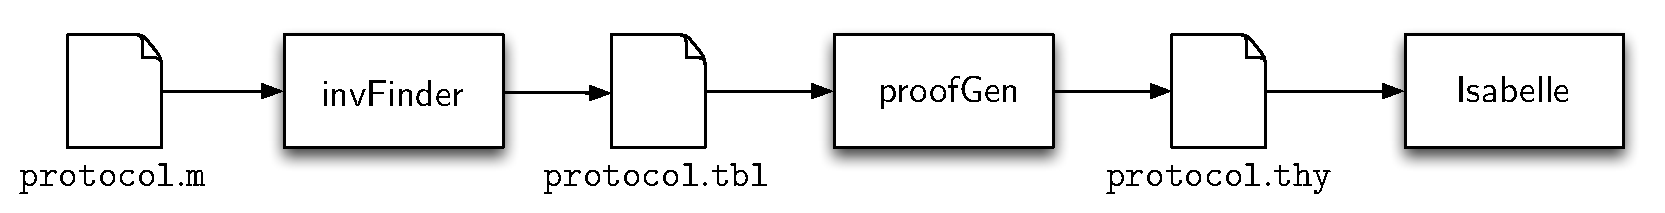
\includegraphics[width=1.0\textwidth]{paraVerifier.pdf}
%\vspace{-2cm}
 \caption{The general architecture of our parameterized
verification}
\label{fig:arch}
\end{figure}
 %\vspace{1cm}
%

%It is the task of {\sf paraVerifier} to construct each one of the
%remaining invariants by checking the causal relation between an
%invariant and a rule instance.


\section{  {\sf invFinder}}
The tool {\sf invFinder} works in a semi-proving and semi-searching
workflow. In an iterating step, it tries to prove some consistent
relation exists between an concrete invariant and a rule, and automatically
generates a new auxiliary invariant if there is no such an invariant
in the current invariant set, and records the corresponding causal
relation information between the current rule and invariant. This
workflow is not finished until no new invariants is created.

\subsection{The InvSearch Algorithm}

The core part of the {\sf invFinder} tool is an algorithm which ....



\begin{algorithm}

\caption{Core Searching Algorithm-I: $InvFinder-I$}\label{alg:invfinder}

\KwIn{$chk$, $tautChk$, $rule$, $inv$, $invs$   }

\KwOut{A formula  option $f$, a new causal relation $rel$}

{
    $g\leftarrow $the guard of rule, $S\leftarrow $the statement of rule\;

    $inv'\leftarrow preCond(inv, S)$\;

    \If{$inv=inv'$}
    {
    $relItem\leftarrow (rule, inv, invRule_2,-)$\;
    \Return $(NONE,  relItem )$\;
    }
    \ElseIf{$tautChk(g\rightarrow inv')=true$}
    {
    $relItem\leftarrow (rule, inv, invRule_1,-)$\;
    \Return $(NONE,  relItem )$\;
    }
    \Else
    {
    $candidates\leftarrow subsets(dualNeg(inv')\wedge g)$\;
    $newInv\leftarrow choose(chk,candidates)$\;
    $relItem\leftarrow (rule, inv, invRule_3,newInv)$\;
    \If{$isNew(newInv,  invs)$}
    {
    $newInv \leftarrow  normalize(newInv)$\;%$ and insert it into the head of $newInvs$\;
    \Return $(SOME(newInv),   relItem )$\;
    }
    \Else{\Return $(NONE,  relItem )$\;}
    }
}

%}

\end{algorithm}


%{\sf invFinder} is implemented by FL, which is an excellent STE-tool
The above core algorithm needs to call two oracles. The first one, denoted by {\tt chk}, checks whether a ground formula is an invariant in a given small reference model of the protocol. Such an oracle can be implemented by firstly translating the formula into a formula in SMV, and then calling SMV to check whether it is an invariant. The second oracle, denoted by
{\tt tautChk}, checks whether a formula is a tautology. Such a tautology checker is implemented by translating the formula into a form in the SMT (abbreviation for SAT Modulo Theories) format, and then calls an SMT solver such as Z3 to check it.

Besides the two oracles which are passed as parameters, there are also other parameters in the algorithm {\tt InvFinder}, including a rule instance $rule$, an invariant $inv$, a sets of invariants $invs$, and a set of causal relations $casRel$. The algorithm {\tt InvFinder} searches for new invariants and    constructs the causal relation between the rule instance $r$ and the invariant $inv$. The sets $invs$  and the set $casRel$ stores causal relations constructed up to now.%  The above function {\sf findInvsFromRule} tries to find new
%invariants and construct the causal relation between the rule
%instance $rule$. %The statement {\tt
%cond => te|fe} is an abbreviation of the if-then-else expression
%that if $cond$ is true then $te$ else $fe$.
%Parameters $newInvs$, $invs$, and $casRel$ are new invariants, invariants, and all the
%causal relations constructed up to now, the above oracle functions
%are also passed as parameters.  % Causal relations  are still not
%checked between the ones in $newInvs$ and rules.
The returned result
is a pair of the newly found invariant(if found),    and causal relation item.
%

After computing the pre-condition $ inv'$, which is the weakest precondition of the input formula $inv$ w.r.t. $S$, and takes further operations according to the cases it faces with:
{\sf invFinder-I} performs case analysis on $inv'$:

\begin{description}
\item[(1)]  if $ inv=inv'$,
 which means that statement $S$ does not change $inv$, then no new invariant is created, and  new causal
relation item marked with tag {\tt invHoldForRule$_2$} is recorded
between $rule$ and $inv$, but at this moment there are no new
invariants to be added; for instance, let $ rule=\mathsf{crit} (3)$,  $ inv=\mathsf{mutualInv}(1,2)$, thus
$inv'=\mathsf{preCond}(S,inv)=inv$, then a pair  $ (\mathsf{NONE}, ( crit(3), inv, \mathsf{invHoldForRule}_2,\_))$ will be returned, where $NONE$ means no new invariant formula is returned.

\item[(2)] Secondly, if $\mathsf{ tautChk}$ verifies that $g \longrightarrow inv'$ is a tautology, then  no new invariant is created, and
the new causal relation item marked with tag
$ \mathsf{invHoldForRule}_1$ is recorded between $rule$ and $inv$. For instance, let $rule=\mathsf{crit}(2)$, $inv=\mathsf{invOnX}_1(1)$,
 $inv'=\mathsf{preCond}(S,inv)=\neg(\mathsf{false }\eqc \mathsf{true} \andc n[1] \eqc \mathsf{C})$, obviously, $
g \longrightarrow_C inv'$ holds forever because $inv'$ is always evaluated true,
 thus a pair $(\mathsf{NONE},  (\mathsf{crit}(2), inv, \mathsf{invHoldForRule}_1,\_))$ will be returned.


 \item[(3)] Thirdly, if neither of the above two cases holds, then a new auxiliary invariant $newInv$ will be constructed, which will make the causal relation $ \mathsf{invHoldForRule}_3$  to hold.


The construction of the auxiliary invariant is introduced better after giving some definitions. A formula $f$ can be composed into a set of sub-formulas $f_i$, denoted as $decompose(f)$, such that each $f_i$ is not of a conjunction form and $f$ is semantically equivalent to $f_1 \wedge f_2 \wedge ... \wedge f_N$. For a formula $f$, we use $subsets(f)$ to denote the power set of $decompose(f)$, which contains all subsets of $decompose(f)$.


A proper formula is chosen from the candidate set $subsets(dualNeg(inv')\wedge g)$ to construct a new invariant $newInv$. This is accomplished by the {\tt choose} function, which calls the oracle {\tt chk} to verify whether a formula is an invariant in the given reference model. After $newInv$ is chosen, the function $isNew$ checks whether this invariant is new w.r.t. $newInvs$ or $invs$. If this is the case, the invariant will be normalized, and then be  added into $newInvs$, and the new causal relation item marked with tag {\tt invRule$_3$} will be added into the causal relations. Here, the meaning of the word ``new" is modulo to the symmetry relation. For instance,   $\mathsf{mutualInv}(1,2)$ is equivalent to
$\mathsf{mutualInv}(2,1)$ in a symmetry view. The $\mathsf{ normalize}$ function normalizes the numbering order of the use of parameters in the invariant $inv$.
The result formula should be   a normal form, whose parameters
  always start from 1, and increase one by one if there are more
  parameters. Namely,  $\negc (x\eqc\mathsf{true} \andc n[1]\eqc\mathsf{C})$ is normalized, but
  $\negc (x\eqc\mathsf{true} \andc n[2]\eqc\mathsf{C})$  not.    Let $ invs=\emptyset$, $ rule=\mathsf{crit}(1)$, $ inv=\mathsf{mutualInv}(1,2)$,
$ inv'= \mathsf{preCond}(S,inv)=\negc(true\eqc true \andc n[2]\eqc C)$, from all the subsets of $\{n[1]\eqc T, x\eqc true, n[2]\eqc C\}$, the $ \mathsf{choose}$ oracle selects the subset $\{ x=true, n[2]\eqc C\}$ combines all the item in this candidate, then constructs a new invariant $ \neg(x\eqc true \andc
   n[2]=\eqc C)$. After   normalization, the new invariant   $\neg(x=true \wedge
   n[1]\eqc C)$  and  a  relation item $ ((crit(1),   \mathsf{invHoldForRule}_3, invs)$ will be returned.


\end{description}



%The main body of {\sf paraVerifier}'s algorithm iteratively calls
%the function {\sf findInvsFromRule}  by instantiating each
%parameterized rule with different actual parameters of the finite
%reference protocol model. This procedure is finished until no more
%5new invariants can be created.
There are three key technique points in our invariant candidate choosing policy. Recalling that our candidate choosing problem can be formulated as follows: Among a set $S$ of invariant formulas, we need choose a set $S_1$ of formulas from $S$ such that $S_1$ is the minimal set that satifies $\neg \bigwedge S_1$ is an invariant. Meanwhile, for any formula set $S_2$ such that $|S_2|<|S_1|$, s $\neg \bigwedge S_2$ is not an invariant.
\begin{itemize}
\item An oracle {\tt chk  } will check whether a formula $\neg \bigwedge S_1$ is an invariant. In our implementation, the oracle firstly tries to use a reachable set of a simplified reference protocol instance within a small size $L$  to check the validity of the formula if each variable of $\neg \wedge S_1$ exists in this small instance; otherwise, the oracle uses MURPHI or  BMC feature of NUSMV to rule out the non-invariant formulas within another reference protocol instance where all the variables of $\neg \bigwedge S_1$ exists, and regard the formula as an invariant if MURPHI or  BMC procedure time-outs. For verification of a complex protocol, the combination of the two choosing strategies are important because we cann't solely enumerate a complete reachable set of a reference protocol instance even with a small size where all the variables of $\neg \bigwedge S_1$ exists. For FLASH with data manipulations, it is not feasible to enumerate a complete reachable set of a reference protocol instance with size $3$  to check the validity of the  candidate; however we can use the  reachable set of a reference instance of simplified FLASH protocol without data manipulations with size $3$ to conjecture control properties, and use the second strategy from a full FLASH protocol with data with size $3$ to guess the properties on data properties or control properties involving a parameter which is greater than L.

\item Choosing policy are done in an augmenting way. Firstly, we initialize $size=1$ choose a set $S$ with $|S_1|=size$, if {\tt chk $S_1$}, then stops; otherwise increases $size$; this process repeats until $S=S_1$ or  {\tt chk $S_1$}.

\item Some heuristics choosing policy can be done which are basing on some experience in this field. For instance, if the pre-condition {\tt inv'} contains only a parameterized variable $v$ with a parameter $i$, then $f$ in $S$ will be choosen with some priority which $v$ occurs in $f$; if we still cann't choose such a formula $f$. We can  try to find another formula $g$ which contains a global variable $v'$ which will be assigned with a new value in the statement of the rule. $\{ f,g \}$ usually is the desired set $S_1$.
\end{itemize}


\subsection{The Parameter Instantiation Policy}

According to a parameter instantiation policy, main body of {\sf invFinder} generates a group of actual parameters to instantiate a parameterized rule $pr$ into a set of actual rules $R$, and call Algorithm \ref{alg:invfinder} to compute new invariant and causal relation between each rule   $r\in rs$ and an invariant formula $inv$. In order to formulate our parameter instantiation policy, we need introduce the concept of permutation modulo to symmetry relation $\sim_m^n$,  and a quotient set of $\mathsf{perms}_{m}^{n}$ (the set of all $n$-permutations of $m$) under the  relation.
\begin{definition}
Let $m$ and $n$ be two natural numbers, where $m \le n$,  $L$ and $L'$ are two lists which stand for two  $n$-permutations of $m$,
\begin{enumerate}
\item
$L \sim_m^n L' \equiv (|L| =|L'|) \wedge (\forall i. i<|L| \wedge L_i \le m-n \longrightarrow L_i=L'_i)$.

%\item$[[L]]_{m}^{n} \equiv \{L'. L \in \mathsf{perms}_{m}^{n} \wedge L \sim_m^n L'\}$.

\item $\mathsf{semiP}(m,n,S)\equiv (\forall  L \in \mathsf{perms}_{m}^{n} \exists  L' \in S. L \sim_m^n L' ) \wedge (\forall  L\in S. \forall L'\in S. L \neq L' \longrightarrow \neg  (L \sim_m^n L' )$.

\item    A set $S$ is called a quotient of the set $\mathsf{perms}_{m}^{n}$ under the relation $\sim_m^n$ if and only if    $\mathsf{semiP}(m,n,S)$.
\end{enumerate}
\end{definition}

For instance, let $m=5$, $n=2$, $[1,2]\not\sim_5^2[2,1]$, $[1,3]\sim_5^2[1,4]$ and  $[5,4]\sim_5^2 [4,5]$. It is easy to see that, $[[1,2],[1,3],[2,1],[2,3],[3,1],[3,2],[3,4]]$ is a quotient set of $\mathsf{perms}_{m}^{n}$ under $\sim_5^2$.

If $m>0$,   $\mathsf{perms}_{m}^{1}$ is the quotient set of itself under $\sim_m^1$.

The following algorithm computes a quotient of $\mathsf{perms}_{m}^{n}$.
\begin{algorithm}

\caption{Computing quotient of $\mathsf{perms}_{m}^{n}$: $cmpSemiperm$}\label{alg:invfinder}

\KwIn{$m$, $n$     }

\KwOut{A permutation set $S$}

{


    %$inv'\leftarrow preCond(inv, S)$\;

    \If{$m=0 \vee n=0$  }
    {
    $S\leftarrow \emptyset $\;
    \Return $S$\;
    }
    \Else
    {
    $S_0\leftarrow \mathsf{perms}_m^n$\;
     $S\leftarrow \emptyset $\;
     \While{$S_0 \neq \emptyset$}
      {$L \leftarrow \mathsf{hd}(S_0)$\;
       $S_0 \leftarrow \mathsf{tl}(S_0)$\;
       \If{$\mathsf{find}(\sim_m^n(L), S)=NONE$}
        { $S\leftarrow S@[L]$\;}
      }
    \Return $S$\;
    }
}

%}

\end{algorithm}

{\bf Our Parameter Instantiation Policy:}
Let $cinv$  be a concrete invariant, $pr$ be a parameterized rule, $\mathsf{aPNumOfInv}(cinv) $ be the number of actual parameters occurring in $cinv$, and $\mathsf{fpNumOfRule}(pr) $  be the number of formal parameters occurring in $pr$,  our policy is to compute the set  $\mathsf{cmpSemiperm}(\mathsf{aPNumOfInv}(cinv)+\mathsf{fpNumOfRule}(pr),\mathsf{fpNumOfRule}(pr) )$, and use elements of it as a group of parameters to instantiate $pr$ into a set $R$ of actual rules.




Now we discuss the completeness of our parameter instantiation policy. How many instantiations are needed? Here the underlying
instantiation principle should guarantee that each typical proof
case by comparing parameters occurring in a rule and an invariant in parameterized protocol instance,  should be covered by a sampling case in our
parameter instantiation policy. That is to say, if we regard the finite
instantiations as samplings, we must guarantee that
 the samples are enough to   be generalized in {\sf proofGen}
to parameterized forms  to finish  parameterized proofs. Here we firstly explain the concept of ``typical proof
case by comparing parameters occurring in a rule and an invariant".  Let $LR=[2]$, $LI=[1,2]$, we compare an element in $LR$ with another of $LI$, $LR_1 = LI_2$ is a formula characterizing the comparation between the first element in $LR$ with the second element in $LI$. Now let us define
\begin{definition}
let $LR \in \mathsf{perms}_N^{|LR|}$ and $LI \in \mathsf{perms}_N^{|LI|}$ are two permutations s.t. $0<|LR|\le N$ and $0<|LI|\le N$
\begin{enumerate}
\item $\mathsf{equality}(LR,LI,i,j) \equiv LR_i = LI_j$.
\item $LR' \in \mathsf{perms}_{N'}^{\mathsf|LR|)}$ and $LI' \in \mathsf{perms}_{N'}^{|LI'|}$ are two permutations s.t. $0<|LR'|\le N$ and $0<|LI'|\le N$ and $|LR|=|LR'|$, and $|LI|=|LI'|$, $\mathsf{reflection}((LR,LI),(LR',LI')) \equiv \forall i \le \mathsf{len}(LR) j\le \mathsf{len}(LI). (\mathsf{equality}(LR,LI,i,j) \leftrightarrow \mathsf{equality}(LR',LI',i,j))$

\end{enumerate}
\end{definition}

$\mathsf{reflection}((LR,LI),(LR',LI'))$ means that each equality comparation between $LR_i$ and $LI_j$ is reflected by that between $LR'_i$ and $LI'_j$. Namely, if we do case analysis by comparing elements in $LR$ and in $LI$, the case pattern are the same with that by comparing those in $LR'$ and in $LI'$.


Recall our parameter instantiation policy:  for a parameterized rule $pR$, a parameterized   formula $pinv$, we only use an identical permutation $ID$ to instantiate $pinv$, and
permutations in $\mathsf{cmpSemiperm}(\mathsf{len}(LR)+\mathsf{len}(LI),\mathsf{len}(LR))$ to instantiate $pR$. We are interested in the completeness of parameter instantiation policy:    let $LR$ and $LI$ are actual parameters to instantiate $pR$ and $pInv$ respectively, the case analysis pattern between $LR$ and  $LI$ can be reflected by that between some $LR'$ and $ID$, where $LR' \in \mathsf{cmpSemiperm}(\mathsf{len}(LR)+\mathsf{len}(LI),\mathsf{len}(LR))$, $ID$ is a permutation with the same length with $LI$. Luckily, the following lemma gives a positive answer.



%relation $LR_i=LI_j$  can be kept by a comparing  $LR'_i=ID_j$, where $LR'$ is a permutation in  $\mathsf{cmpSemiperm}(\mathsf{len}(LR)+\mathsf{len}(LI),\mathsf{len}(LR))$, $ID$ is identical permutation such that $ID_i=i$.
\begin{lemma}[completeness of parameter instantiation]\label{lemma:completeness}
let $LR \in \mathsf{perms}_N^{\mathsf{len}(LR)}$ and $LI \in \mathsf{perms}_N^{\mathsf{len}(LI)}$ are two permutations s.t. $\mathsf{len}(LR)>0$ and $\mathsf{len}(LI)>0$ and $\mathsf{len}(LR) \le N$  and $\mathsf{len}(LI) \le N$, let $ID$ be an identical permutation which has the same length with $LI$, there exists a permutation $LR' \in \mathsf{cmpSemiperm}(\mathsf{len}(LR)+\mathsf{len}(LI),\mathsf{len}(LR))$ s.t. $\mathsf{reflection}((LR,LI),(LR',ID))$.
\end{lemma}

Here we use two examples to explain this lemma. Let $LR=[2]$, $LI=[2,1]$, there exists $LR'=[1]\in \mathsf{cmpSemiperm}(3,1)$ s.t. $reflect((LR,LI),(LR',ID))$; let $LI=[5,6]$, there exists $LR'=[3]\in \mathsf{cmpSemiperm}(3,1)$ s.t. $\mathsf{reflect}((LR,LI),(LR',ID))$.


\subsection{The Top-level Algorithm?}


New invariant and causal relation between each rule   $r\in R$ and an invariant formula $cinv$ will be computed. The algorithm of parameter instantiation to the parameterized rule and calling {\sf invFinder-I} to search  auxiliary invariants are listed as follows:

\begin{algorithm}

\caption{parameter instantiations: invFinder-II }\label{alg:parameterInstantiate}

\KwIn{parameterized rule $pr$,  a concrete invariant $cinv$, two formula set $invs$ and $newInvs$, a relation set $rel$ }

\KwOut{  two formula set $invs'$ and $newInvs'$, a relation set $rel'$ }

{  $ni\leftarrow \mathsf{aPNumOfInv}(cinv) $\;
   $nr \leftarrow \mathsf{fpNumOfRule}(pr)$\;

   $S \leftarrow \mathsf{cmpSemiperm}(ni+nr,nr)$\;
   $invs' \leftarrow invs$\;
   $newInvs' \leftarrow newInvs$\;
   $rel' \leftarrow rel$\;
     \While{$S  \neq \emptyset$}
     {
       $L \leftarrow \mathsf{hd}(S )$\;
        $S  \leftarrow \mathsf{tl}(S )$\;
        $r \leftarrow \mathsf{apply}(pr,L)$\;
        $result \leftarrow  \mathsf{InvFinder-I}(chk,tauto,r,cinv,invs')$\;
      $rel' \leftarrow rel'@\mathsf{snd}(result)$\;
       \If{$\mathsf{fst}(result) \neq NONE$}
        {$newInv \leftarrow \mathsf{getReal}(\mathsf{fst}(result)) $\;
        $invs' \leftarrow invs'@[newInv]$\;
         $newInvs' \leftarrow newInvs'@[newInv]$\;
        }
     }
    \Return $invs', newInvs'$  and  $rel'$
}



\end{algorithm}


 The output of the {\sf invFinder}, which is stored in file {\tt mutual.tbl},  is shown in Table
\ref{label-ground-causal relation}. In the table,  each line records the    index of a normalized   invariant, name of a parameterized rule, the rule
  parameters to instantiate the rule, a causal relation between
  the ground invariant and a kind of causal relation which involves the kind and proper formulas
  $f'$   in need (which are used to construct
      causal relations $\mathsf{invHoldForRule}_3$). The auxiliary invariants found by {\sf invFinder} includes: $\mathsf{inv_2}  \equiv  \negc (\mathsf{x} \eqc true  \andc  n[1]=C)$, $\mathsf{inv_3}    \equiv \negc  ( n[1]=C \andc n[2]=E)$,
$\mathsf{inv_4}  \equiv  \negc (x \eqc \mathsf{true}  \andc  n[1]\eqc \mathsf{E})$,   $\mathsf{inv_5}    \equiv \negc  ( n[1]\eqc \mathsf{C} \andc n[2] \eqc \mathsf{C})$.



 \begin{table}[!t]
\centering \caption{A fragment of output of {\sf invFinder}}\label{label-ground-causal relation} % {\tt
%simpMutual.tbl}
\begin{tabular}{|c|c|c|c|c|  }
\hline
  rule& ruleParas&inv&causal relation &   f'  \\
\hline
  .. & ..&.. &..&.. \\

\hline
  crit  & [1]&mutualInv(1,2)& invHoldForRule3 &invOnX$_1$(2) \\
\hline
  crit &[2]& mutualInv(1,2)& invHoldForRule3 &invOnX$_1$(1)  \\
\hline
  crit & [3]& mutualInv(1,2) & invHoldForRule2  & \\
\hline
  .. & ..&.. &..&.. \\

\hline
  crit  & [1]&invOnX$_1$(1) & invHoldForRule1 &\_ \\
\hline
  crit &[2]& invOnX$_1$(1) & invHoldForRule1 &\_  \\
\hline
\end{tabular}
\end{table}



 Here we list  explain  the meanings of the five lines:
   \begin{itemize}
   \item   $\mathsf{apNumOfcInv}(\mathsf{invOnX_1}(1))=1$ and $\mathsf{fpNumOfRule}(\mathsf{crit})=1$, there are two lines, in which  [1] and [2] are used to instantiate $\mathsf{crit}$  respectively. The sampling case $\mathsf{crit}(1)$ and $\mathsf{invOnX_1}( 1)$ in the reference instance represents a parameterized case
    $\mathsf{invOnX_1}(\iInv_1)$ and $\mathsf{crit}( iR_1)$ where $iR_1=\iInv_1$ in the parameterized instance; the sampling case
    $\mathsf{crit}(2)$ and $\mathsf{invOnX_1}( 1)$ in the reference instance represents a parameterized case $\mathsf{invOnX_1}(\iInv_1)$ and $\mathsf{crit}( iR_1)$ where $ iR_1\ne \iInv_1 $ in the parameterized instance. In any $N-$parameterized instance of the $\mathsf{mutualEx}$ protocol, the cases $iR_1=\iInv_1$ and  $ iR_1\ne \iInv_1 $  completely partitions all the possible cases if we compare $\iR_1$ and $\iInv_1$.

   \item  $\mathsf{apNumOfcInv}(\mathsf{mutualInv}(1,2))=2$ and $\mathsf{fpNumOfRule}(\mathsf{crit})=1$, there are three lines, in which  [1], [2] and [3] are used to instantiate $\mathsf{crit}$  respectively. The sampling case $\mathsf{crit}(1)$ and $\mathsf{mutualInv}(1,2)$ in the reference instance represents a parameterized case
    $\mathsf{mutualInv}(\iInv_1,\iInv_2)$ and $\mathsf{crit}( iR_1)$ where $iR_1=\iInv_1$ in the parameterized instance; the sampling case
    $\mathsf{crit}(2)$ and $\mathsf{mutualInv}(1,2)$ in the reference instance represents a parameterized case $\mathsf{mutualInv}(\iInv_1,\iInv_2)$ and $\mathsf{crit}( iR_1)$ where $ iR_1= \iInv_2 $ in the parameterized instance, and the sampling case $\mathsf{crit}(3)$ and $\mathsf{mutualInv}(1,2)$ in the reference instance represents a parameterized case
    $\mathsf{mutualInv}(\iInv_1,\iInv_2)$ and $\mathsf{crit}( iR_1)$ where $iR_1 \ne \iInv_1$ and $iR_1 \ne \iInv_2$in the parameterized instance. In any $N-$parameterized instance of the $\mathsf{mutualEx}$ protocol, the cases $iR_1=\iInv_1$,  $iR_1=\iInv_2$ and  $ iR_1\ne \iInv_1 \wedge iR_1\ne \iInv_2 $  completely partitions all the possible cases if we compare $\iR_1$ and $\iInv_1$ and $\iInv_2$.
    \end{itemize}
%In order to  explain the idea of  finite sampling, we need recall our proof in Example \ref{caseSimp}. The typical proof pattern is based on case analysis  by %comparing the rule parameters such as $iR$ and invariant parameters such as $i_1$ and $i_2$. We also recall that the invariants searched by {\tt invFinder} are %always in a normal form, whose parameters
%  always start from 1, and increase one by one if there are more
 % parameters. The last, but not the least, is the symmetry of the cache coherence we exploit. Namely, a sampling case is one representative of an equivalence class  modulo to some symmetry relation.
The above  only informally explains the correspondence between concrete case and the accordingly  parameterized case by two instances, and we will formally define the correspondence and the generalization strategy which transforms   the concrete cases searched by the {\sf invFinder} into parameterized cases which will be used in Isabelle proof.



%\section{Generalization}

\section{Generalization}
Intuitively, generalization means that a concrete index (formula or rule) is a representation of set of concrete indice (formulas or rules), which can be formalized  by a symbolic index (formula or rules) with side conditions specified by the constraint formulas. These constraint formulas can be formalized in our modelling languages in turn.    In order to formally define the parameterized instance, we need extend our modelling language:

\begin{specification}
datatype indexType = scalar nat | formal string \\

datatype varType=Ident  string | Para varType indexType | Field  varType string\\

datatype valueType=enum string string |index indexType | boolV bool | symb string\\

%type\_synonym paramDefType= paramDef indexType valueType\\
%type\_synonym forallForm::paramDefType list $\Rightarrow$  formula  \\



%fun exitsForm::paramDefType list $\Rightarrow$ formula \\



\end{specification}

\begin{definition}
Let $LR$ be a permutation s.t. $\mathsf{len}(LR)>0$, which represents a list of actual parameters to instantiate a rule,    let $ID$  be an identical permutation $\mathsf{len}(ID)>0$,  which  represents a list of actual parameters to instantiate a normalized invariant, we define:
\begin{enumerate}
\item symbolic equality  between $LR_i$ and $LI_j$: $symbEq(LR,LI,i,j)\equiv$ if $equality(LR,LI,i,j)$ then $\mathtt{\iR_i} = \mathtt{\iInv_j}$ else $\neg(\mathtt{\iR_i} = \mathtt{\iInv_j})$
    
\item symbolic case on a parameter $i$ between $LR_i$ and $LI$ : $symbcaseI(LR,LI,i)\equiv $if there exists a unique position $j$ s.t. $equality(LR,LI,i,j)$, then   $symbEq(LR,LI,i,j)$, else $forallForm(length(LI),pf)$, where $pf(j)= symbEq(LR,LI,i,j)$
    
\item symbolic case  between $LR$ and $LI$ : $symbcaseI(LR,LI )\equiv forallForm(length(LR),pf)$, , where $pf(i)= symbcaseI(LR,LI,i )$
    
\item symbolic partition decided by a $LRS$ and $LI$, where $LRS$ is a set of permutation with the same length: $partition(LRS,LI) \equiv existsForm(length(LRS),pf)$,  where $pf(i)= symbcase(LRS_i,LI)$
    
\end{enumerate}    
\end{definition}

$symbEq(LR,LI,i,j)$ defines a symbolic formula according to the condition $equality(LR,LI,i,j)$, which represents the semantics of the equality between $LR_i$ and $LI_j$; $symbEq(LR,LI,i)$  a symbolic formula equality matching conditions between $LR_i$  and all $LI_j$ such that $j \le length(LI)$; $symbcaseI(LR,LI )$ a subcase decided by all $LR_i$  and all $LI_j$; $partition(LRS,LI)$  is a disjunction of sub-cases $symbcase(LRS_i,LI )$.  Recall the examples in the previous section:
\begin{itemize}
\item when   $LI=[1]$ is a list of parameters occuring in $invOnX_1(1)$ 
\begin{itemize}
  \item $LR=[1]$ are the actual parameters to instantiate $crit$, $symbEq(LR,LI,1,1)=\mathtt{\iR_1} = \mathtt{\iInv_1}$, $symbcase(LR,LI)=symbcaseI(LR,LI,1)=\mathtt{\iR_1} = \mathtt{\iInv_1}$.
    
  \item  $LR=[2]$ are the actual parameters to instantiate $crit$, $symbEq(LR,LI,1,1)=\neg(\mathtt{\iR_1} = \mathtt{\iInv_1})$, $symbcase(LR,LI)=symbcase(LR,LI,1)=\neg(\mathtt{\iR_1} = \mathtt{\iInv_1})$
      
   \item let $LRS=[[1],[2]]$, $partition(LRS,LI)= (\mathtt{\iR_1} = \mathtt{\iInv_1}) \vee \neg(\mathtt{\iR_1} = \mathtt{\iInv_1})$
\end{itemize}     
\item when   $LI=[1,2]$ is a list of parameters occuring in $mutualEx(1,2)$  
\begin{itemize} 

  \item $LR=[1]$ are the actual parameters to instantiate $crit$, $symbEq(LR,LI,1,1)=\mathtt{\iR_1} = \mathtt{\iInv_1}$, $symbcase(LR,LI,1)=\mathtt{\iR_1} = \mathtt{\iInv_1}$.

  \item  $LR=[2]$ are the actual parameters to instantiate $crit$, $symbEq(LR,LI,1,1)=\neg(\mathtt{\iR_1} = \mathtt{\iInv_1})$, $symbcase(LR,LI,1)=\mathtt{\iR_1} = \mathtt{\iInv_2})$ becasue $LR_1=LI_2$.
      
      
 \item  $LR=[3]$ are the actual parameters to instantiate $crit$, $symbEq(LR,LI,1,1)=\neg(\mathtt{\iR_1} = \mathtt{\iInv_1})$, $symbcase(LR,LI)=symbcaseI(LR,LI,1)=\neg(\mathtt{\iR_1} = \mathtt{\iInv_1}) \wedge \neg(\mathtt{\iR_1} = \mathtt{\iInv_2})$ because neither $LR_1=LI_1$ nor $LR_1=LI_2$.
 
  \item let $LRS=[[1],[2],[3]]$, $partition(LRS,LI)= (\mathtt{\iR_1} = \mathtt{\iInv_1}) \vee (\mathtt{\iR_1} = \mathtt{\iInv_2}) \vee (\neg(\mathtt{\iR_1} = \mathtt{\iInv_1}) \wedge \neg(\mathtt{\iR_1} = \mathtt{\iInv_1}))$
\end{itemize}     
\end{itemize} 

Note that $partition(LRS,LI)$ is a complete partition if it is a tautology. In the above example, the two partitions are both complete. 

\begin{definition}
Let $N$ be a symbolic value representing a size of a parameterized instance of a protocol, $iInd$ be a string,  we define:
\begin{enumerate}
\item model constraint-I: $modelConstrI(N,iInd,i) \equiv \mathtt{iInd_i} \le N$.
\item model constraint: $modelConstr(N,iInd,L) \equiv forallForm(pf,length(L))$, where $pf(i)=modelConstrI(N,iInd,i)$.
\end{enumerate}
\end{definition}

For instance, $modelConstrI(N,``\iR", 1)=\mathtt{iR_1} \le N$; $modelConstr(N,``\iInv",[1,2])=\mathtt{iInv_1} \le N \wedge \mathtt{iInv_2} \le N$. 

\begin{definition}
let $iInd$ be a string, 
\begin{enumerate}
\item difference constraint between parameter $\mathtt{iInd}_i$ and $\mathtt{iInd}_j$: $diff(iInd,i,j) \equiv \neg (\mathtt{iInd}_i = \mathtt{iInd}_j)$.
\item mutual difference constraint: $mutualDiff(iInd,L) \equiv \bigwedge S$, where $S=\{f. f=diff(iInd,i,j)~ and~ i\le len(L) ~and~ j \le len(L)~ and ~i < j\}$.
\end{enumerate}
\end{definition}
For instance, $diff( ``\iInv", 1,2)=\neg(\mathtt{\iInv_1} = \mathtt{\iInv_2})$; $mutualDiff( ``\iInv",[1,2])=\neg (\mathtt{iInv}_1 =\mathtt{ iInv}_2)$; $mutualDiff( ``\iInv",[1,2,3])=\neg (\mathtt{iInv}_1 = \mathtt{iInv}_2) \wedge \neg (\mathtt{iInv}_1 = \mathtt{iInv}_3) \wedge \neg (\mathtt{iInv}_2 = \mathtt{iInv}_3)$.
%-------------------------------------------------------------------------
\section{Automatical generation of Isabelle proof by {\tt proofGen}}
%-------------------------------------------------------------------------

A formal model in a theorem prover like Isabelle
includes the definitions of constants and rules and invariants,
lemmas, and proofs. An overview of the transformation strategy is
shown in Fig \ref{fig:mapping} from a protocol instance in FL to
 the one in Isabelle.


 \begin{figure}[!ht]
% \centering %
 %\vspace{-0.8cm}
\includegraphics[width=1.0\textwidth]{isabelleScript.pdf}
%\vspace{-0.5cm}
 \caption{An overview of an Isabelle proof}
\label{fig:arch}
\end{figure}
% \vspace{1cm}
\subsubsection{Generating definitions of formal  rules and actual rules in a $N-$ parameterized instance}
A formal definition of an invariant and all actual invariants of  $N-$parameterized instance of $\mathsf{mutual}$ protocol is shown as follow:\\

\begin{specification}

 definition pinv4::nat $\Rightarrow$ formula   where [simp]:\\

       pinv4 \iInv1 $\equiv$\\

      neg ( andForm ( eqn ( IVar (Ident ''x'') )  ( Const true ))   \\

          ( eqn ( IVar ( Para ''n'' \iInv1) )  ( Const E)) )  \\

definition invariants::nat $\Rightarrow$ formula set  where [simp] :\\
invariants N$\equiv$ \{f. $\exists$ \iInv1 \iInv2. \iInv1 $\le$ N $\wedge$ \iInv2 $\le$ N $\wedge$ \iInv1 $\ne$ \iInv2 $\wedge$  f = pinv1 \iInv1 \iInv2  $\vee$ \\
 $\exists$ \iInv1. \iInv1 $\le$ N $\wedge$  f = pinv2 \iInv1   $\vee$\\
$\exists$ \iInv1 \iInv2. \iInv1 $\le$ N $\wedge$ \iInv2 $\le$ N $\wedge$ \iInv1 $\ne$ \iInv2 $\wedge$  f = pinv3 \iInv1 \iInv2  $\vee$\\
$\exists$ \iInv1. \iInv1 $\le$ N $\wedge$  f = pinv4 \iInv1  $\vee$\\
$\exists$ \iInv1 \iInv2. \iInv1 $\le$ N $\wedge$ \iInv2 $\le$ N $\wedge$ \iInv1 $\ne$ \iInv2 $\wedge$ f = pinv5 \iInv1 \iInv2  $\vee$   \}\\


\end{specification}

 For a record {\tt symbForm invName f num  sideConstraint} in the invariant table $symbInvTab$, the generation of its formal definition in Isabelle is rather straight-forward: {\tt invName} is used to the name of this invariant  this definition such as {\tt pinv4}, {\tt num} is used to define the type of this invariant formula such as {\tt nat $\Rightarrow$ formula}, and  {\tt f} is used to define the body of definition in Isabelle.  Besides, we also need to define the set of all the actual formulas of invariants
 in the $N-$parameterized instance by {\tt invariants N}, each element of which can be an invariant formula instance. Notice that the constraints(assumptions) in the case condition such as {\tt $\exists$ \iInv1 \iInv2. \iInv1 $\le$ N $\wedge$ \iInv2 $\le$ N $\wedge$ \iInv1 $\ne$ \iInv2 $\wedge$  f = pinv1 \iInv1 \iInv2 } comes from two parts:  (1) the facts that all parameters of this invariant should be less than the parameter $N$; (2) the constraints from  {\tt sideConstraint}, which specifies that the mutual difference between two parameters.

\begin{specification}
letrec strsCat sepStr []=""\\
\alt strsCat sepStr [str]=str\\
\alt strsCat sepStr (str\#strs)=str \cat sepStr \cat  (strsCat sepStr strs)\\
 %strLs =itlist ($\lambda$ str1.$\lambda$ str2.str1 \cat sepStr \cat str2) strLs ""
let asmLess str SN i=str$_i$ \cat "$\le$ " \cat SN\\
let asmsGen str sN len=strsCat  (asmLess \iInv sN  ))  (1 upto len) " "\\
let asmsLookUp tab name fieldName=map form2Isabelle (fieldName (tbl\_element tab name))\\
let constraintGen symbInvs invName =\\
\twoSpaces   let asmsLessOnInv=asmsGen \iInv~ "N"~ lenPInv in\\
\twoSpaces  let asmsMutualDiffOnInv=asmsLookUp symbInvs invName gFldName in\\
\twoSpaces strsCat "$\wedge$"  (asmsLessOnInv@asmsMutualDiffOnInv)   \\

let parasGen temp len =
  strsCat " " (map (index2Isabelle temp) ( 1 upto len)\\

let invParasGen lenPInv=parasGen \iInv lenPInv  \\

let frmDisj symbInvs invName=\\

\twoSpaces val (symbInv invN f  lenPInv gf)=tbl\_element symbInvs invName in\\
\twoSpaces if (lenPInv=0) then "f=invName"\\
\twoSpaces else let constraint=constraintGen symbInvs invName in\\
\twoSpaces let parasStr=invParasGen lenPInv in\\
\twoSpaces sprintf "$\exists$ \%s. \%s $\wedge$ f=\%s \%s" parasStr constraint invName parasStr\\

let frmsDisjs symbInvs  =\\
\twoSpaces strCat "$\vee$" (tbl\_map frmDisj symbInvs)\\

let actualInvsDefGen symbInvs=\\
\twoSpaces sprintf "definition invariants::nat $\Rightarrow$ formula set  where [simp] :\\
invariants N $\equiv$ \{f. \%s\}" (frmsDisjs symbInvs)\\
%let asmsMutualDiffOnInv=asmsLookUp symbInvs invName gFldName in
\end{specification}

In order to define the function to generate the definition all the actual invariants in the $N$-parameterized instance, we define a function {\tt strsCat}, which concats a list of strings with a delimeter string {\tt sepStr}. {\tt asmLess} returns   a constraint that a parameter is less or equal to $N$. For instance, {\tt asmLess \iInv~"N"  1="\iInv1$\le$N"}. {\tt parasGen} generates a string of parameters, which will be applied to a name of a invariant formula (or a rule). For instance, {\tt parasGen \iInv~ 2="\iInv1 \iInv2"}. {\tt asmsLookUp} generates constraints of the mutual difference between two parameters, which can be looked up by the invariant name from the field  {\tt gFldName} storeded in a record;  {\tt frmDisj} generates a formula in Isabelle to specify a possible form of an invariant formula. For instance,  {\tt frmDisj symbInvs pInv1="$\exists$ \iInv1 \iInv2. \iInv1 $\le$ N $\wedge$ \iInv2 $\le$ N $\wedge$ \iInv1 $\ne$ \iInv2 $\wedge$  f = pInv1 \iInv1 \iInv2"},\\  {\tt frmsDisjs} generates all the cases of the possible form of an invariant formula. With these predefined functions, {\tt actualInvsDefGen} generates the definition of all the invariant formulas: {\tt invariants N}.
%   For instance, let $gInv_4\equiv \neg (x=true \wedge n[1]=C)$, we define
%   a formal parameterized formula:
%  $pinv_4~i_1 \equiv
%  (x=true \wedge n[i_1]=C)$,
%  and $ex1P~N~(\lambda i.pInv~i)$ is all the actual formulas which are symmetric to $gInv$ in the N-parameterized
%  instance of the protocol, and Spec \ref{} shows its Isabelle syntax of the invariant $pinv_4$ generated by {\tt proofGen}.
% {\tt  invariants N} is the set of all the actual rules. %;  for $gInv= (n[1]=C \wedge n[2]=C)$, we define an
%  $pInv~i_1~i_2=(n[i_1]=C \wedge n[i_2]=C)$, and $ex2P~N~(\lambda i~j.pInv~i~j)$ is all the formulas
%  which are symmetric to $gInv$ in the N-paramterized instance of the
 % protocol. At last, we can define the set of all the auxiliary
 % invariants, which will be proved to be consistent with all the
 % rule.
% $ \mathsf{invariants} ~N \equiv \{f. ex1P~ N ~(\lambda i.  f= inv_{11}~ i)  ...\vee ex1P ~N ~(\lambda i.  f = inv_{1m}~ i )
%  \vee
% (ex2P~ N ~\lambda i ~j.  f= inv_{21}~ i~j)  ...\vee ex2P~ N ~(\lambda i~j.  f =inv_{2n}~ i~j
% ) \vee
%(ex3P~ N ~\lambda i ~j~k.  f= inv_{31}~ i~j~k)  ...\vee ex3P~ N
%~(\lambda i~j~k.  f =inv_{3o}~ i~j~k\}$, where $inv_{1i}$,
%$inv_{2j}$, and $inv_{3k}$ are formal invariant formulas with one,
%two three formal parameters respectively.  .


  Similar to the generation of   formulas, accordingly we can generate all the formal definition of rules and the actual rules used in the $N-$parameterized instance by the table $symbRules$.

\subsubsection{Generating lemmas for causal relation between rules and invariants}
  Now we discuss how to use records on {\tt crit} and {\tt inv1} in the table $symbCausalTab$ to generate a lemma to prove causal relation hold between some rule $pr$ and some invarianr $inv_j$,
which will be applied in the proof of main lemma. An  example lemma
{\tt critVsinv$_1$} and its proof in Isabelle in the {\tt mutualEx} protocol, is illustrated as follows:


\begin{specification}
1lemma critVsinv1:\\
2  assumes  a1: $\exists$ \iR1. \iR1 $\le$ N $\wedge$ r=crit \iR1 and \\
  a2: $\exists$  \iInv1 \iInv2. \iInv1 $\le$ N $\wedge$ \iInv2 $\le$ N $\wedge$ \iInv1 $\neq$ \iInv2 $\wedge$ f=inv1  \iInv1 \iInv2\\
3  shows  invHoldForRule s f r (invariants
  N)\\
4  proof -\\
   from a1 obtain \iR1 where a1:\iR1 $\le$ N $\wedge$ r=crit \iR1 \\
   by blast\\
   from a2 obtain \iInv1 \iInv2 where \\
   a2: \iInv1 $\le$ N $\wedge$ \iInv2 $\le$ N $\wedge$ \iInv1 $\neq$ \iInv2 $\wedge$ f=inv1  \iInv1 \iInv2\\
   by blast \\
5  have iR1=\iInv1 $\vee$ \iR1=\iInv2 $\vee$ (\iR1 $\ne$ \iInv1 $\wedge$  \iR1 $\ne$ \iInv2) by auto\\

6  moreover\{assume  b1:\iR1=\iInv1\\
7  \twoSpaces have invHoldForRule3 s f r (invariants N)\\
 \twoSpaces  \twoSpaces   proof(cut\_tac a1 a2 b1, simp, rule\_tac x=$\negc$ (x=true $\andc$ n[\iInv2]=C)  in exI,auto)qed\\
8  \twoSpaces then have invHoldForRule s f r
(invariants
  N)
by auto\}\\

9  moreover\{assume  b1:iR1=\iInv2\\
10 \twoSpaces have invHoldForRule3 s f r (invariants N)\\
 \twoSpaces \twoSpaces   proof(cut\_tac a1 a2 b1, simp, rule\_tac x=$\negc$ (x=true $\andc$ n[\iInv1]=C  in exI,auto)qed\\
11 \twoSpaces then have invHoldForRule s f r (invariants
  N)
by auto\}\\

12   moreover\{assume  b1:(\iR1 $\ne$  \iInv1 $\wedge$   \iR1 $\ne$  \iInv2)\\
13 \twoSpaces have invHoldForRule2 s f r  \\
  \twoSpaces \twoSpaces  proof(cut\_tac a1 a2 b1,  auto) qed\\
14 \twoSpaces then have invHoldForRule s f r
(invariants
  N)
by auto\} \\

15ultimately show invHoldForRule s f r
(invariants N) by blast\\
16qed\\
\end{specification}

An lemma such as {\tt critVsinv1}  is generated by collecting all the records on the invariant {\tt inv1} and rule {\tt crit} in the table $symbRules$.
Line 2 are assumptions on the parameters of the invariant and rule, which come from two parts: (1) assumption {\tt a1} specifies that {\tt r} is a rule obtained by instantiating {\tt crit} with a parameter {\tt \iR1}. (2) assumption {\tt a1} specifies that {\tt f} is a formula obtained by instantiating {\tt inv1} with  parameters {\tt \iInv1} and {\tt \iInv2}.
 %(1) the facts that all parameters of this invariant should be less than the parameter $N$; %(2) the facts that all parameters of this invariant should be less than the parameter $N$; (3) the constraints of he mutual difference between parameters of the invariant (rule), which can %be looked up in the field of those records  from the table $symbInvTab$ ($symbRuleTab$) by the invariant (rule) name {\tt inv1} ({\tt crit}), which specifies that the mutual difference %between two parameters.
Line 4 are two typical forward-style proof pattern which fixes local variables such as {\tt \iR1} and new facts such as {\tt a1: iR1 $\le$ N $\wedge$ r=crit \iR1}. From line 5, the remaining parts of the proof is a typically readable one in Isar style \cite{}, which uses calculation
reasoning such as {\tt moreover} and {\tt ultimately} to do  case analysis.
Line 5 splits cases of $iR1$ into all possible cases by comparing
{\tt \iR1} with {\tt \iInv1} and {\tt \iInv2}, which is the disjunction of all the {\tt caseFld} fields of these records. Lines 6-14  proves    these cases one by one: Lines 6-8 proves the case where {\tt iR1=\iInv1}; Lines 6-8 proves the case where {\tt iR1=\iInv2}; Lines 12-14 the case   where neither {\tt iR1=\iInv1} nor {\tt iR1=\iInv2}. Each proof of a subcase is done in a block {\tt moreover b1:asm1 proof1}, the {\tt ultimately}  proof command in line 15 concludes by summing up all the subcases.

%The aforementioned proof can be generated by instantiate the following pattern by replacing {\tt rule},
%{\tt inv}, {\tt proof1}, {\tt proof2}, {\tt proof3} with {\tt crit} and the detail proof lines 7-8, 11-12, and 14-15 respectively.
%This pattern works for each pair of a parameterized rule with two parameters and an invariant
%with two parameters.
%pattern of case analysis on the parameters  is determined by the number of parameters of
%the invariant and rule, which can be formalized by a proof template. Lines 1-5, 6, 9, 10, 13, 14, 17 18,19 can be resused by replacing the names of rule and
% invariant respectively.
%Detail proofs such as lines  7, 10, 13 are generated according to the lines on {\tt crit} and {\tt inv1} in Table \ref{}. The mapping is based on the symmetry mapping. Recall the  parameters instantiation policies we discussed in section \ref{},. {\t proof1} at line 7 is according with line in Table because the latter case is the representive of the former case in the sense of symmetry. These proofs are composed of two parts: a middle result to show which kind of causal relation should be choose to prove, then from this the conclusion can be obtained immediately.
%Thus  in  {\t proof1} should introduce a middle result $\mathsf{invHoldForRule_{3}}$, whose proof needs an existence construction by providing an auxiliary invariant formula {\tt $\neg$ (x=true $\wedge$ n[i2]=C}. {\t proof2} can be constructed similarly. {\t proof3} chooses $\mathsf{invHoldForRule_{2}}$ to prove,  , an {\tt auto} command is enough because such a goal can be solved automatically in Isabelle.




\begin{specification}
%letrec strsCat sepStr []=""\\
%\alt strsCat sepStr [str]=str\\
%\alt strsCat sepStr (str\#strs)=str \cat sepStr \cat  (strsCat sepStr strs)\\
 %strLs =itlist ($\lambda$ str1.$\lambda$ str2.str1 \cat sepStr \cat str2) strLs ""
%let asmLess str SN i=str$_i$ \cat "\dbRight<le> " \cat SN\\
%let asmsGen str sN len=itlist (\lambda i.\lambda str2.str2 \cat "" \cat (asmLess str SN i)) (map (\lambda i. str_i) (1 upto len)) " "\\
%let asmsLookUp tab name fieldName=map form2Isabelle (fieldName (tbl\_element tab name))\\
%let namedAsmTrans asmStr i="a" \cat (nat2str i) \cat ":" \cat asmStr\\
%let allNamedAsmsGen sN lenPInv lenPRule ruleName inVName symbRules symbInvs =\\
%\twoSpaces   let asmsLessOnInv=asmsGen \iInv sN lenPInv in\\
%\twoSpaces  let asmsLessOnRule=asmsGen iRule sN lenPRule in \\
%\twoSpaces  let asmsMutualDiffOnInv=asmsLookUp symbInvs invName gFldName in\\
%\twoSpaces  let asmsMutualDiffOnRule=asmsLookUp symbRules ruleName gFldName in\\
%\twoSpaces  let asmsOnInv=asmsLessOnInv@asmsMutualDiffOnInv in\\
%\twoSpaces  let asmsOnRule=asmsLessOnRule@asmsMutualDiffOnRule in\\
%\twoSpaces   let allAsms=asmsLessOnInv@asmsLessOnRule@asmsMutualDiffOnInv@asmsMutualDiffOnRule in\\
%\twoSpaces   let allNamedAsms=map ($\lambda$ (asmStr,i). namedAsmTrans asmStr i) (zip allAsms (1 upto (length %allAsms))) in\\
%\twoSpaces     strsCat " and " allNamedAsms\\




let rulePrarasGen lenPRule=parasGen iR lenPRule \\

let oneMoreBranch asmDepth asmForm proofStr=\\
\twoSpaces let asmName=asmDepth2Name asmDepth in\\
\twoSpaces sprintf\\
\twoSpaces "moreover\{assume  \%s:\%s  \%s    \} "\\
\twoSpaces (asmName, asmForm, proofStr)\\

\\
%let moreOversOnIfBra asmDepth causalLines =


let symbCausalRec2Case  symbRec=\\
\twoSpaces  val (symbLine rnmae invName caseF holdTag formOpt)=symbRec in\\
\twoSpaces     form2Isabelle caseF\\

let symbCausalRecs2Allcases symbRecs=\\
\twoSpaces    (map symbCausalRec2Case symbRecs)\\
\\
let proof3Gen caseF invHold3f=\\
%\twoSpaces sprintf\\
%\twoSpaces "moreover\{assume  b1:\%s\\
\twoSpaces have invHoldForRule3 f r (invariants N)\\
\twoSpaces  \twoSpaces   proof(simp, rule\_tac x=\%s  in exI,auto)qed\\
%\twoSpaces \twoSpaces then have invHoldForRule s f r (invariants   N)  by auto"\\
%\twoSpaces (form2Isabelle caseF, \\
\twoSpaces (form2Isabelle invHold3f)\\


let symbCausalRec2OneMore symbRec=\\
\twoSpaces  val (symbLine rnmae invName caseF  holdTag formOpt)=symbRec in\\
\twoSpaces  let proof=   if (holdTag=invHold1) then \\
\twoSpaces      proof1Gen   caseF\\
\twoSpaces     else if  (holdTag=invHold2) then \\
\twoSpaces      proof2Gen   caseF\\
\twoSpaces     else proof3Gen   caseF invHold3f in\\
\twoSpaces  let asm= form2Isabelle caseF in \\
\twoSpaces      oneMoreBranch 1 asm proof \\

let symbCausalRecs2AllMores symbRecs=\\
\twoSpaces    (map symbCausalRec2Proof symbRecs)\\
\\

let doCaseAnalzProofs casSplittings moreovers concluding depth=\\
\twoSpaces if (length casSplittings=1) then sprintf\\
\twoSpaces "\%s\\
\twoSpaces \twoSpaces then \%s \%s by auto"\\
\twoSpaces \twoSpaces (moreovers!1,if depth=1 then "show" else "have",  concluding)\\
\twoSpaces else sprintf\\
\twoSpaces \twoSpaces  " have \%s  by auto\\
\twoSpaces \twoSpaces         \%s\\
\twoSpaces \twoSpaces        ultimately \%s \%s by auto"\\
\twoSpaces     (strsCat "$\vee$" casSplittings, strsCat " "  moreovers,\\
\twoSpaces     if depth=1 then "show" else "have",  concluding)\\
\\
let lemmaOnCausalRuleInv ruleName invName symbRules symbInvs symCausalTab  =\\
\twoSpaces let allSymbRecs=tbl\_element (ruleName \cat invName)) symCausalTab in\\
\twoSpaces let lenPInv=paraNumFld  (tbl\_element symbInvs  invName) in\\
\twoSpaces let lenPRule=paraNumFld  (tbl\_element symbRules  ruleName) in\\
\twoSpaces let asms1="a1:"  \cat (frmDisj symbInvs invName)   in\\
\twoSpaces let asms2="a2:"  \cat (ruleDisj symbInvs ruleName)   in\\
\twoSpaces let asms=asms1 \cat asms2 in\\
\twoSpaces let invParas=invParasGen lenPInv in\\
\twoSpaces let constraintOnInv= constraintGen symbInvs invName in\\
\twoSpaces let ruleParas=rulePrarasGen lenPRule in\\
\twoSpaces let constraintOnRule= constraintGen symbRules ruleName in\\
\twoSpaces let allCaseSplits=symbCausalRecs2Allcases allSymbRecs in\\
\twoSpaces let moreovers=symbCausalRecs2AllMores allSymbRecs in\\
\twoSpaces let concluding="invHoldForRule s f r (invariants   N)" in\\
\twoSpaces let proof=doCaseAnalzProofs allCaseSplits moreovers concluding 1 in\\
\twoSpaces let obtain1= if (lenPInv=0) then ""\\
\twoSpaces else sprintf "from a1 obtain  \%s where a1:\%s $\wedge$ f=\%s \%s by auto"\\
 \twoSpaces           (invParas,  constraintOnInv, invName, invParas) in\\
\twoSpaces let obtain2= if (lenRInv=0) then ""\\
\twoSpaces else sprintf from a2 obtain  \%s where a2:\%s $\wedge$ r=\%s \%s by auto"\\
 \twoSpaces           (ruleParas,  constraintOnRule, ruleName, ruleParas) in
\twoSpaces sprintf\\

\twoSpaces"lemma \%sVs\%s:\\
%2  assumes  a2: iR $\le$ N and a3: i1 $\le$ N and a4: i2 $\le$ N\\ generations assumptions
\twoSpaces assumes \%s\\
\twoSpaces  shows  invHoldForRule s f r (invariants   N)\\
\twoSpaces  proof -
\twoSpaces \%s~ \%s~  \%s

\twoSpaces qed"\\

\twoSpaces (ruleName, inVName, asms, obtain1, obtain2, proof) \\
\end{specification}


Function {\tt lemmaOnCausalRuleInv ruleName invName  symbRules symbInvs symCausalTab} returns a lemma on causal relation between  an invariant and a rule named {\tt  invName} and {\tt  ruleName} respectively.
The generation procedure is according with the parts of the lemma such as {\tt critVsinv1}. The name of the lemma is decided by the {\tt ruleName} and {\tt invName} respectively.  {\tt allSymbRecs } are all symbolic causal relation records on {\tt  invName} and {\tt  ruleName},
 then  {\tt lenPInv} and {\tt lenPRule} which are numbers of the parameters of the invariant formula and rule. The assumptions part {\tt asms} of the generated lemma is the combination of  {\tt asm1} and {\tt asm2}, which are  assumptions on the invariant and the rule respectively. Recall that the proof is an Isar forwarding style: two {\tt obtain} proof commands; then proof commands of case analysis: {\tt have cases   moreover\{case1 proof1\} ...  moreover\{casen proofn\} ultimately concludes}. If the parameter numbers of the invariant formula is 0, then we need not such an {\tt obtain} proof command and we directly use the fact {\tt a1} in the assumption of the lemma, otherwise an obtain pproof command is generated according to the number of the parameters of the invariant. {obtain2} proof command is generated similarly.   {\tt proof} is generated  by calling function {\tt doCaseAnalzProofs allCaseSplits moreovers concluding}. {\tt } is the cases in the case splitting proof command is the disjuction of all the formulas, which are generated from {\tt caseF} field by calling {\tt symbCausalRec2Case} function. {\tt moreovers} are all subproofs of all sub-cases. {\tt Concluding} is the conclusion of the proof. In each sub-proof in one element of {\tt moreovers}, its content is corresponding to one a symbolic casual relation record {\tt symbRec}:   the assumption of the case is from the {\tt caseF} field of  {\tt symbRec}. Its proof is generated from the by calling {\tt symbCausalRec2Proof symbRec}, which generates a kind of proof in Isabelle according to  the field {\tt holdTag} {\tt symbRec}: if the tag of {\tt holdTag} is 1(2,3), then kind 1 (2,3) proof are generated accordingly. Here we list the most complex one: {\tt proof3Gen ruleName invName f}, which generates a proof which is according with {\tt invHoldType3} such as lines 6-8, and {\tt f} is another invariant formula which is needed to construct the {\tt invHoldType3} causal relation.


 % {\tt allSymbRecs } are all symbolic causal relation records on {\tt  invName} and {\tt  ruleName},
% then  {\tt lenPInv} and {\tt lenPRule} which are numbers of the parameters of the invariant formula and rule, then {\tt asms} which are the assumptions part of the lemma such as line 2, {\tt allDisjuncts} the case analysis between the parameters of invariant and rule such as line 5, {\tt allSubProofs} all the proofs of the subcases such as lines 6-14, then fill all these into the blanks of the templates to generate the lemma.


% {\tt namedAsmTrans asm i} adds a name "ai:" to a string of assumption in order to construct a named assumption. {\tt allNamedAsmsGen} generates all the aformentioned  four kinds of assumptions of the lemma in the previous paragrapgh: {\tt asmsLessOnInv} is according with (1) types of assumptions; {\tt asmsLessOnRule} (2) types of assumptions;  {\tt asmsMutualDiffOnInv} (3) types of assumptions; and {\tt asmsMutualDiffOnRule} (4) types of assumptions. After naming any one assumption with a name, {\tt allNamedAsmsGen} returns all the named assumptions which are conned by {\tt and} operator. {\tt symbCausalRec2Proof symbRec} generates a kind of proof in Isabelle according to a symbolic casual relation record {\tt symbRec}: if the tag of {\tt holdTag} is 1(2,3), then kind 1 (2,3) proof are generated accordingly. Here we list the most complex one: {\tt proof3Gen ruleName invName f}, which generates a proof which is according with {\tt invHoldType3} such as lines 6-8, and {\tt f} is another invariant formula which is needed to construct the {\tt invHoldType3} causal relation.
%\twoSpaces  let asmsLessOnRule=asmsGen iRule sN lenPRule in \\
%\twoSpaces  let asmsMutualDiffOnInv=asmsLookUp symbInvs invName gFldName in\\
%\twoSpaces  let asmsMutualDiffOnRule
\subsection{Definitions and lemmas on initial states}

In this section, we discuss the definition on the initial state of the protocol, and the lemmas specifying that each invariant formula hold at the initial state.

A typical Isabelle definition on the initial state of the protocol is as follows:

\begin{specification}
definition initSpec0::nat $\Rightarrow$ formula where [simp]:\\
initSpec0 N $\equiv$ (forallForm (down N) (\% i . (eqn (IVar (Para (Ident ''n'') i)) (Const I))))\\

definition initSpec1::formula where [simp]:\\
initSpec1  $\equiv$ (eqn (IVar (Ident ''x'')) (Const true))\\

definition allInitSpecs::nat \<Rightarrow> formula list where [simp]:\\
allInitSpecs N $\equiv$ [(initSpec0 N),(initSpec1 )]\\

lemma iniImply\_inv4:
assumes a1: ($\exists$\iInv1. \iInv1$\le$N$\wedge$f=inv4 \iInv1)\\
and a2: formEval (andList (allInitSpecs N)) s\\
shows formEval f s\\
 using a1 a2 by auto\\
\end{specification}

{\tt initSpec0} and {\tt initSpec1} specifies the assignments on each variable {\tt n[i]} where {\tt i $\le$ N} and {\tt x}. The  specifications of the initial state is the list of all the specification definition on related state variables. Lemma {\tt iniImply\_inv4} simply specifies that the invariant formula {\tt inv4} holds at a state {\tt s} which satisfies the conjunction of the   specification of the initial state. Isabelle's {\tt auto} method can solve this goal automatically. Other lemmas specifying that other invariant formulas hold at the initial state are similar. These lemmas are prepared for the first part of the application of the consistency lemma in the main theorem.


The generation of the above code is straightforward: definitions of the specification of initial state variables in Isabelle is a direct syntax transformation from the internal represetation of tool {\tt proofGen} to Isabelle. Generation of lemma {\tt iniImply\_inv4} is the calling the following  function by paasing {\tt invName} with {\tt inv4}.

\begin{specification}
let lemmaInitGenOnInv invName=\\
\twoSpaces let constraintOnInv= constraintGen symbInvs invName in\\
\twoSpaces sprintf \\
\twoSpaces "lemma iniImply\_\%s:\\
\twoSpaces assumes a1: \%s\\
\twoSpaces and a2: formEval (andList (allInitSpecs N)) s\\
\twoSpaces shows formEval f s\\
\twoSpaces using a1 a2 by auto\\"
\twoSpaces     invName   constraintOnInv\\

\end{specification}


\subsubsection{Generating proofs for the main lemma}

%-------------------------------------------------------------------------
At last, we discuss how to create automatically the proof for the main lemma, which depends
 on the applying the lemmas which are created in subsection \ref{sec:genOfIsabelleProof}.  The consistency lemma is our
main weapon to prove, which requires proving two parts of
obligations.



\begin{description}
\item[(1)] For any invariant $inv \in (\mathsf{invariants} ~N) $,  any
state $s$, if $ini$ is evaluated true at state $s$, then $inv$ is
evaluated true at state $s$.
\item[(2)]  For any invariant $inv \in (\mathsf{invariants} ~N)$, any $r$ in rule set
$ \mathsf{rules} ~N$ , one of the causal relations
$\mathsf{invHoldForRule}_{1-3}$ holds.
\end{description}
%
%Proof of Part (1) is  simple. %%For an invariant
%$inv=\mathsf{implyForm}~ant~cons$ in $invs$, we only need to prove
%that either $ant$ is evaluated as false or $cons$ is evaluated true
%at an initial state $s$ in order to prove $\models
%~inv~s$. Such a proof  can be automatically solved by Isabelle's
%$\mathsf{auto}$ command.
An overview of a formal proof  generated by {\tt
proofGen} is illustrated as follows: it is mainly divided into two parts, which are according with the two proof obligations generated by  applying the consitency lemma. Part 1  does case analysis on the form of the invariant formulas {\tt f}.  In each case where {\tt f} is a kind of invariant named by {\tt invName},  and the goal is solved by applying rule {\tt iniImply\_invName}.  Part 2  is based on the two levels of case analysis on the form of rules and the invariants.
 In the first level, we do case analysis on the form of rules, then we do case analysis on the form of invariants.
For a case on proving the existence of casual relation between {\tt ruleName} and {\tt invName}, we solve the subgoal by the lemma  {\tt ruleNameVsinvName} such as {\tt critVsInv1}.


\begin{specification}
lemma main:
  $\isasymlbrakk$  s$\in$ reachableSet \{andList (allInitSpecs N)\} (rules N); 0<N$\isasymrbrakk$\\
  $\Longrightarrow$ $\forall$ inv. inv $\in$ (invariants N) $\longrightarrow$ formEval inv s\\
proof(rule consistentLemma)\\
  show consistent (invariants N) \{andList (allInitSpecs N)\} (rules N)\\
 proof(cut\_tac a1, unfold consistent\_def,rule conjI)\\
   show  $\forall$inv ini s. inv $\in$ (invariants N)
$\longrightarrow$ ini $\in$\{andList (allInitSpecs N)\}$\longrightarrow$formEval
ini s $\longrightarrow$ formEval inv s\\
proof((rule allI)+,(rule impI)+)\\
\twoSpaces   fix inv ini s\\
\twoSpaces   assume b1:inv $\in$ (invariants N) \\
\twoSpaces     and b2:ini $\in$ \{andList (allInitSpecs N)\}  and b3:formEval ini s\\
\twoSpaces   have b4:\\
%\twoSpaces    proof -\\
\twoSpaces     have        ($\exists$ \iInv1 \iInv2. \iInv1 $\le$ N $\wedge$ \iInv2 $\le$ N $\wedge$ \iInv1 $\ne$ \iInv2 $\wedge$  f = inv1 \iInv1 \iInv2)$\vee$ \\
\twoSpaces\oneSpace($\exists$ \iInv1.   \iInv1 $\le$ N $\wedge$    f = inv2 \iInv1 )$\vee$ \\
\twoSpaces\oneSpace ......\\
\twoSpaces\oneSpace ($\exists$ \iInv1 \iInv2. \iInv1 $\le$ N $\wedge$ \iInv2 $\le$ N $\wedge$ \iInv1 $\ne$ \iInv2 $\wedge$  f = inv5 \iInv1 \iInv2)  \\
\twoSpaces\twoSpaces   ~by (cut$\_$tac b1, simp )\\

\twoSpaces\twoSpaces   moreover\\
\twoSpaces\oneSpace\twoSpaces$\{$assume c1: $\exists$ \iInv1 \iInv2. \iInv1 $\le$ N $\wedge$ \iInv2 $\le$ N $\wedge$ \iInv1 $\ne$ \iInv2 $\wedge$  f = inv1 \iInv1 \iInv2\\
  \twoSpaces\twoSpaces   have formEval inv s\\
  \twoSpaces\twoSpaces     apply (rule iniImply\_inv\_1)\\
   \twoSpaces\twoSpaces    apply (cut\_tac c1, assumption)\\
  \twoSpaces\twoSpaces     by (cut\_tac b4, simp)  \}\\
\twoSpaces\twoSpaces           ......\\
\twoSpaces\twoSpaces   moreover\\
\twoSpaces\oneSpace\twoSpaces$\{$assume d1: $\exists$ \iInv1 \iInv2. \iInv1 $\le$ N $\wedge$ \iInv2 $\le$ N $\wedge$ \iInv1 $\ne$ \iInv2 $\wedge$  f = inv5 \iInv1 \iInv2\\
\twoSpaces\twoSpaces    have formEval inv s\\
 \twoSpaces\twoSpaces      apply (rule iniImply\_inv\_5)\\
  \twoSpaces\twoSpaces     apply (cut\_tac c1, assumption)\\
 \twoSpaces\twoSpaces      by (cut\_tac b4, simp)  \}\\
\twoSpaces    ultimately show formEval inv s   by blast\\

    qed\\

next   show  $\forall$inv r. inv $\in$ invariants N$\longrightarrow$
 r $\in$rules N$\longrightarrow$invHoldForRule inv r (invariants N) \\

   proof((rule allI)+,(rule impI)+)\\
\twoSpaces      fix f r \\
\twoSpaces         assume b1: f $\in$ invariants N  and b2:r $\in$ rules N\\

\twoSpaces      have c1: ($\exists$ iR1. iR1 $\le$ N $\wedge$ r=exit iR1)$\vee$\\
\twoSpaces  ($\exists$ iR1. iR1 $\le$ N $\wedge$ r=idle iR1)$\vee$ \\
\twoSpaces   ($\exists$ iR1. iR1 $\le$ N $\wedge$ r=crit iR1) $\vee$ \\
\twoSpaces  ($\exists$ iR1. iR1 $\le$ N $\wedge$ r=try iR1)\\
\twoSpaces\twoSpaces         by(cut$\_$tac  b2,auto)\\
\twoSpaces moreover\\
\twoSpaces\oneSpace $\{$assume c1: $\exists$ iR1. iR1 $\le$ N $\wedge$ r=exit iR1 \\

\twoSpaces\oneSpace have d1:   ($\exists$ \iInv1 \iInv2. \iInv1 $\le$ N $\wedge$ \iInv2 $\le$ N $\wedge$ \iInv1 $\ne$ \iInv2 $\wedge$  f = inv1 \iInv1 \iInv2)$\vee$ \\
\twoSpaces\oneSpace($\exists$ \iInv1.   \iInv1 $\le$ N $\wedge$    f = inv2 \iInv1 )$\vee$ \\
\twoSpaces\oneSpace ......\\
\twoSpaces\oneSpace ($\exists$ \iInv1 \iInv2. \iInv1 $\le$ N $\wedge$ \iInv2 $\le$ N $\wedge$ \iInv1 $\ne$ \iInv2 $\wedge$  f = inv5 \iInv1 \iInv2)  \\
\twoSpaces\twoSpaces   ~by (cut$\_$tac b1, simp )\\

\twoSpaces\oneSpace\twoSpaces  moreover\\
\twoSpaces\oneSpace\twoSpaces$\{$assume d1: $\exists$ \iInv1 \iInv2. \iInv1 $\le$ N $\wedge$ \iInv2 $\le$ N $\wedge$ \iInv1 $\ne$ \iInv2 $\wedge$  f = inv1 \iInv1 \iInv2\\


\twoSpaces\oneSpace \twoSpaces  have invHoldForRule f r (invariants N) \\
\twoSpaces\twoSpaces\twoSpaces         by(cut$\_$tac  c1 d1, metis exitVsInv1)\}\\
\twoSpaces\twoSpaces\twoSpaces  ......\\
\twoSpaces\oneSpace\twoSpaces moreover\\
\twoSpaces\oneSpace\twoSpaces      $\{$assume d1: $\exists$ \iInv1 \iInv2. \iInv1 $\le$ N $\wedge$ \iInv2 $\le$ N $\wedge$ \iInv1 $\ne$ \iInv2 $\wedge$  f = inv5 \iInv1 \iInv2\\

\twoSpaces\oneSpace\twoSpaces ......~~~~          \\
\twoSpaces\oneSpace \twoSpaces  have invHoldForRule s f r (invariants N) \\

\twoSpaces\twoSpaces\twoSpaces     by(cut$\_$tac c1 d1, simp) $\}$\\


\twoSpaces\oneSpace \twoSpaces ultimately have invHoldForRule s f r (invariants N) \\

\twoSpaces\twoSpaces\twoSpaces     by blast \\%\}\\
\twoSpaces\twoSpaces\twoSpaces        $\}$\\

\twoSpaces  moreover\\
\twoSpaces\oneSpace  $\{$assume c1: $\exists$ iR1. iR1 $\le$ N $\wedge$ r=idle iR1\\

\twoSpaces\oneSpace \oneSpace  ......\\

\twoSpaces\oneSpace \oneSpace   \}\\
\twoSpaces ......\\
\twoSpaces                   ultimately show invHoldForRule s f r (invariants N) ~~by blast\\
qed\\
qed\\


%next\\
%~~show s $\in$ reachableSet {mutualIni N} (rules N) ~~by (metis
%a1)\\
%
%next.... \\

%qed\\ %end\\
\end{specification}
%\vspace{-0.5cm}
 %in order to verify the cache coherence protocols. Others are straightforward.
%The proof is a typically
%readable one in Isar style \cite{}, which uses calculation
%reasoning such as {\tt moreover} and {\tt ultimately} to do  case analysis on
%the form of rules and the invariants. Lines 1-5 use proper Isabelle
%proof commands to   decompose the main proof goal of forall  and
%implication form,    fix a rule {\tt r} and {\tt inv}, then have two
%assumptions {\tt  b1: inv$\in$ invariants N  and b2:r $\in$ rules
%N}, now we need show the goal {\tt invHoldForRule s f r (invariants
%N)}. line 5 splits cases of $r$ into all possible cases according to
%the definition of $rules~N$. %In order to save space, we adopt the following abbreaviation:
% $\mathsf{ex1P}~ N~ P \equiv \exists i. (i \le N \wedge P~
%i)$, $\mathsf{ex2P}~ N~ P \equiv \exists i~j. (i \le N \wedge j \le
%N \wedge i\ne j \wedge P~ i~j)$, and $\mathsf{ex3P}~ N~ P \equiv
%\exists i~j~k. (i \le N \wedge j \le N \wedge k \le N\wedge i\ne j
%\wedge i\ne k \wedge j\ne k \wedge P~ i~j~k)$.
%Line 6 starts the case analysis on
%$r=r_0$. Line 7 again splits cases of $inv$ into all possible cases
%according to the definition of $invariants~N$. Line 8-10 proves the
%goal at case when $r=exit$ and $inv=inv1$. At line 10,  a  proved
%lemma {\tt exitVsInv1}  is directly applied to solve the proof
%goal.  Similiarly, we can do subproofs on other cases on {\tt inv},
%and finish the proof goal accordingly.
% After finishing the proof of the last case  of $inv=inv5$,
% we finish the proof of the first case $r=exit$. Similarly, we can
% finish the proof goal at
%each subcase on {\tt r}. At  lines 19 and  20 we show we have
%finished the proof goal formally.


\begin{specification}


let genOneMoreOverInPart1 symbInvs invName =\\
\twoSpaces let caseAsm= frmDisj symbInvs invName in\\
\twoSpaces let caseProof=\\
\twoSpaces sprintf "\\
\twoSpaces \twoSpaces      have formEval f s\\
\twoSpaces \twoSpaces      apply (rule iniImply\_\%s)\\
\twoSpaces \twoSpaces      apply (cut\_tac c1, assumption)\\
\twoSpaces \twoSpaces      by (cut\_tac b4, simp)" invName in \\
\twoSpaces oneMoreBranch caseAsm caseProof 1\\

let genProofOfPart1 symbInvs=\\
\twoSpaces  let allCaseSplits=frmDisjs symbInvs in\\
\twoSpaces  let moreovers=map (genOneMoreOverInPart1 symbInvs) symbInvs in\\
\twoSpaces  let concluding="formEval f s" in\\
\twoSpaces  doCaseAnalzProofs allCaseSplits moreovers concluding 1\\

let genOneMoreOverOnInvInPart2 ruleName symbInvs invName =\\
\twoSpaces let caseAsm= frmDisj symbInvs invName in\\
\twoSpaces let caseProof=\\
\twoSpaces sprintf "\\
\twoSpaces \twoSpaces      have invHoldForRule f r (invariants N) \\
\twoSpaces \twoSpaces  by(cut\_tac c1 d1, metis \%sVs\%s) (ruleName, invName) in \\
\twoSpaces oneMoreBranch caseAsm caseProof 3\\


let genOneMoreOverOnRuleInPart2  symbInvs symbRules ruleName =\\
\twoSpaces let caseAsm= ruleDisj symbRules ruleName in\\
\twoSpaces  let allCaseSplits=frmDisjs symbInvs in\\
\twoSpaces  let moreovers=map (genOneMoreOverOnInvInPart2 ruleName symbInvs) symbInvs in\\
\twoSpaces  let concluding="invHoldForRule f r (invariants N) " in\\
\twoSpaces let caseProof=  doCaseAnalzProofs allCaseSplits moreovers concluding 2 in\\
\twoSpaces oneMoreBranch caseAsm caseProof 3\\

let genProofOfPart2 symbInvs symbRules=\\
\twoSpaces  let allCaseSplits=ruleDisjs symbRules in\\
\twoSpaces  let moreovers=map (genOneMoreOverOnRuleInPart2 symbInvs symbRules) symbRules in\\
\twoSpaces  let concluding="invHoldForRule f r (invariants N)" in\\
\twoSpaces  doCaseAnalzProofs allCaseSplits moreovers concluding 1\\



let mainThmGen symbRules symbInvs=\\
\twoSpaces let proof1=genProofOfPart1 symbInvs in\\
\twoSpaces let proof2=genProofOfPart2 symbRules in\\
sprintf\\
"theorem main:\\
  $\isasymlbrakk$  s$\in$ reachableSet \{ mutualIni  N\} (rules N); 0<N$\isasymrbrakk$\\
  $\Longrightarrow$ $\forall$ inv. inv $\in$ (invariants N) $\longrightarrow$ formEval inv s\\
proof(rule consistentLemma)\\
  show consistent (invariants N) \{andList (allInitSpecs N)\} (rules N)\\
 proof(cut\_tac a1, unfold consistent\_def,rule conjI)\\
   show  $\forall$inv ini s. inv $\in$ (invariants N)
$\longrightarrow$ ini $\in$\{andList (allInitSpecs N)\}$\longrightarrow$formEval
ini s $\longrightarrow$ formEval inv s\\
proof((rule allI)+,(rule impI)+)\\
\twoSpaces   fix inv ini s\\
\twoSpaces   assume b1:inv $\in$ (invariants N) \\
\twoSpaces     and b2:ini $\in$ \{andList (allInitSpecs N)\}  and b3:formEval ini s\\
\twoSpaces    \%s
 % show consistent (invariants N) \{mutualIni  N\} (rules N)\\
 % proof(cut\_tac a1, unfold consistent\_def,rule conjI)\\
%~~    show  $\forall$inv ini s. inv $\in$ (invariants N)
%$\longrightarrow$ ini $\in$\{mutualIni  N\}$\longrightarrow$formEval
%ini s $\longrightarrow$ formEval inv s\\
%  ~~ proof((rule allI)+,(rule impI)+)\\
% ~~~~ ......\\
%   ~~~~   fix inv ini s\\
%  ~~~~    assume b1:inv $\in$ (invariants N) \\
%  ~~~~    and b2:ini $\in$
%{mutualIni  N}  and b3:formEval ini s\\
%    ~~~~  show formEval inv s\\
%   ~~~~   proof -\\
%
%   ~~~~~~     have c1:      exLessP N (\%i.  inv= inv1 i) $\vee$exLessP N (\%i.  inv= inv2 i) $\vee$
%    ex2P N (\%i j. inv=inv3 i
%   j) \\$\vee$ ex2P N (\%i j. inv=inv4 i j)$\vee$ex2P N (\%i j. inv=inv5 i j)\\%$\vee$\\
% %  ~~~~~~~~                     ex2P N (\%i j. inv=mutualInv3 i j)\\

%    ~~~~~~       by (cut\_tac b1, simp add:invariants\_def)\\

%     ~~~~~~    moreover\\
%    ~~~~~~    \{assume d1: exLessP N (\%i.  inv= inv1 i)\\
%      ~~~~~~     have formEval inv s\\
%       ~~~~~~~~      by (metis b2 b3 d1 iniImplyInv.verify)\}\\
      % ~~~~~~~~   \}\\
       ~~~~~~~~   ......\\
     % ~~~~~~   moreover\\
     % ~~~~~~   \{assume d1: ex2P N (\%i j.  inv=inv5 i j)\\
     %  ~~~~~~    have formEval inv s\\
     %   ~~~~~~~~     by (metis b2 b3 d1 invInterp5.iniImplyInv)\}\\
       % ~~~~~~ \}\\
    %   ~~~~~~   ultimately show formEval inv s\\
     %   ~~~~~~ ~~   by blast\\

%    ~~~~    qed\\

next   show  $\forall$inv r. inv $\in$ invariants N$\longrightarrow$
 r $\in$rules N$\longrightarrow$invHoldForRule inv r (invariants N) \\

   proof((rule allI)+,(rule impI)+)\\
\twoSpaces      fix f r \\
\twoSpaces         assume b1: f $\in$ invariants N  and b2:r $\in$ rules N\\


\twoSpaces\twoSpaces\%s\\

qed\\
qed"\\

(proof1,proof2)
%next\\
%~~show s $\in$ reachableSet {mutualIni N} (rules N) ~~by (metis
%a1)\\
%
%next.... \\

%qed\\ %end\\
\end{specification}
As demonstrated in the previous proof, the main proof is divided into two parts. Function {\tt genProofOfPart1 symbInvs} generates part 1, which is a case analysis proof structure basing on {\tt symbInvs}. The case splittings in this part is  basing on  the possible form of an invariant formula, which is formalized by {\tt frmDisjs symbInvs}. One subproof in a subcase is returned by {\tt genOneMoreOverInPart1 symbInvs invName}. Function {\tt genProofOfPart2 symbRules} generates part 2, which is a two level of a case analysis proof structure, and the top level is bassed on {\tt symbRules}, and the nested level is based on{\tt symbInvs}. The case splittings in this part is  basing on  the possible form of a rule, which is formalized by {\tt ruleDisjs symbInvs}. One subproof in a subcase at the top level is returned by {\tt genOneMoreOverOnRuleInPart2 symbInvs symbRules ruleName}, which also generates a case analysis proof structure basing on {\tt symbInvs}. The case splittings here is  basing on  the possible form of an invariant formula, which is formalized by {\tt frmDisjs symbInvs}. One subproof in a subcase here is returned by {\tt genOneMoreOverOnInvInPart2 ruleName symbInvs invName}.

%=========================================
\section{Verification products}
%=========================================

After the auxiliary invariants are found,  the formula set $\mathsf{pinvs}~ N$ in Table \ref{} can be used to analyze
 and verify the design  of the protocol. In fact, they gives a complete
logical characterization of the semantics of the protocol. It will gives a deep insight of the protocol. These properties imply correspondence between
control signals or mutual exclusion between control signals. For instance, the intuitive meaning of the invariants is analyzed as follows:

\begin{table}[htbp] \label{Summarization of invariants}
\centering \caption{Summarization of invariants}
\begin{tabular}{|c|c| }
\hline
invariant &  meaning  \\
\hline
$\mathsf{invOnX_1} ~i$& Once some n[i] is set C, the flag x will be set false \\
\hline
$\mathsf{invOnX_2} ~i$&  Once some n[i] is set E, the flag x will be set false \\
\hline
$\mathsf{mutualInv}~ i ~j$ &  the mutual exclusion between n[i]=C and n[j]=C \\
\hline
$\mathsf{aux}_1~ i ~j$ &  the mutual exclusion between n[i]=C and n[j]=E \\
\hline
$\mathsf{aux}_2~ i ~j$ &  the mutual exclusion between n[i]=C and n[j]=E \\
\hline
\end{tabular}
\end{table}
%$\mathsf{invOnX_1} ~i$ specifies that the flag $x$ shows the
%availability of the critical section. Once some node state variable
%$n[i]$ is set $C$ or $E$, $x$ will be set $true$. Formulas
%$\mathsf{mutualInv}~ i ~j$, $\mathsf{aux_1} ~i~j$, and
%$\mathsf{aux_2} ~i~j$ state the mutual exclusion properties between
%a node's $\mathsf{C}(\mathsf{E})$ state and another different node's
%$\mathsf{C}(\mathsf{E})$ state.
The causal relations listed in Table \ref{} only illustrate why the invariants hold forever at each reachable state set.
That is to say, for a rule $r$ and an $inv$ descriibed in a line, one of the three causal relation $\mathsf{invHoldForRule}_{1\_3}$ holds, so an invariant holds after the execution the rule $r$. The Isabelle proof-script formally generalize these causal relation into parameterized form and proved the existence of the  causal relations. At last, a main lemma formally specifies that why the invariants hold forever at any reachable state set, and is formally proved by using the consistency lemma. In this sense, the Isabelle script can be seen as  a formal analysis document. The script contains 2243 line, and and costs more than 56
minutes for Isabelle to check in a 64-bit computing server platform which has a
160-multicore Intel Xeon CPU with 2.40GHz clock speed.


%=========================================
\section{Experiments}
%=========================================
We implement our tool in Forte \cite{Forte}. More experiments are
done including typical bus-snoopy ones such as MESI and MOESI,
 directory-based ones such as  Germanish, and  German protocols. The detail experiment codes and data can
be found in \JP{\cite{LiCache14}}. Each experiment data includes the
${\sf paraVerifier}$ instance, invariant sets found, Isabelle proof
scripts, and the simulation flow graph of one single node. A table
summarizes  our experiments below. Among the benchmarks, the German
protocol   was posted
 as
% Among the benchmarks, a case study is done
%on a directory-based protocol, German protocol, which was posted as
a challenge to the formal verification community by Steven German in
2000. German protocol is a moderate case.
To the best of our knowledge, few people but us give a complete proof to verify
the mutual exclusion  property of the German protocol
 in a theorem prover.  We also have successfully verified the important properties of the FLASH protocol, resulting into an independent and different proof from the literature. As Chou, Mannava, Park pointed out in \cite{}, FLASH is a good benchmark for any proposed method for parameterized verification: ��if the method works on FLASH, then there is a good chance that it will also work on many real-world cache coherence protocols��. Therefore, our approach has reached this most important landmark. From the line on the statistics on the FLASH, we can see the huge resource consumed by this case study. Such a big proof project is also a great challenge to a theorem prover like Isabelle. The total size of the proof scripts for FLASH verification is about 16M, which cann't be directly processed by Isabelle if we put all the proof scripts in a file. A file with 5000k is too large to be processed by Isabelle. Instead we have to divided   the proofs into small pieces, which are processed in some order. Therefore we work out a proof project control script in a {\tt ROOT} file to control the proof sessions. The proof consumptions of resources are according with the complexity of the problems. By the FLASH experiment, we demonstrate that ITP combined with automatic proof generation can handle industry-scale case like FLASH.


\begin{table}[!t] \label{Summarization of experiment results}
\centering
\caption{Verification results on benchmarks.}
\vspace{-2mm}
\begin{tabular}{|c|r|r|r|r|}
\hline
Protocols &  \#rules & \#invariants & time (seconds) & Memory (MB) \\
\hline\hline
MESI & 4& 3 & 0.68 & 11.5  \\
\hline
MOESI &  5& 3 &0.65 & 23.2  \\
\hline
Germanish~\cite{cubicle2011}  & 6&3&0.68 & 23.0   \\
\hline
German~\cite{Chou2004} & 13 & 24 & 4.09 & 26.7   \\
\hline
German with data~\cite{Chou2004} & 15 & 50 & 12.05 & 29.4   \\
\hline
Flash~\cite{Park1996a,McMillan2001} & 73 & 112 & 1457.42 & 169.4   \\
\hline
\end{tabular}
\vspace{-5mm}
\end{table}

%=========================================
\section{Conclusion}
%=========================================
Within {\sf paraVerifier},
our automatic framework for parameterized verification of cache coherence protocol,
(1) instead of directly proving the invariants of a protocol by induction, we propose a general
proof method based on the consistency lemma to decompose the proof goal into a number of small ones;
(2) instead of proving the decomposed subgoals by hand,
we automatically generate proofs for them based on the information computed in a small protocol instance.\footnote{Technical details
of {\sf paraVerifier} will be made available in a technical report.}

As we demonstrate in this work, combining theorem proving with
automatic proof generation is promising in the field of formal
verification of industrial protocols. Theorem proving can guarantee the rigorousness of the verification results,
while automatic proof generation can release the burden of human interaction.

%Our case studies on cache coherence protocols are typical examples
%to illustrate the guiding principle of {\sf paraVerifier}. The
% consistency lemma based on the induction approach, is the
%core of our work, which gives the heuristics to guide the tool
% to search invariants. Instead of ``invisible invariants in previous work
% (see e.g,~\cite{Pnueli2001}, our invariants are visible,
% which can be further refined to precisely
% analyze the correctness of the protocol both in theoretical and practical aspects.

\bibliographystyle{splncsnat}
\bibliography{gste,cache,refer}
\end{document}
